%%%%%%%%%%%%%%%%%%%%%%%%%%%%%%%%%%%%%%%%%
% Stylish Article
% LaTeX Template
% Version 2.1 (1/10/15)
%
% This template has been downloaded from:
% http://www.LaTeXTemplates.com
%
% Original author:
% Mathias Legrand (legrand.mathias@gmail.com) 
% With extensive modifications by:
% Vel (vel@latextemplates.com)
%
% License:
% CC BY-NC-SA 3.0 (http://creativecommons.org/licenses/by-nc-sa/3.0/)
%
%%%%%%%%%%%%%%%%%%%%%%%%%%%%%%%%%%%%%%%%%

%----------------------------------------------------------------------------------------
%	PACKAGES AND OTHER DOCUMENT CONFIGURATIONS
%----------------------------------------------------------------------------------------

\documentclass[fleqn,10pt]{SelfArx} % Document font size and equations flushed left

\usepackage[portuguese]{babel} % Specify a different language here - english by default
% \usepackage{lipsum} % Required to insert dummy text. To be removed otherwise
% \usepackage{url} % Required to insert dummy text. To be removed otherwise
\usepackage{balance}

\usepackage{hyperref}
\usepackage{mathptmx}
\usepackage{graphicx}
\usepackage{times}
\usepackage{textcomp}
\usepackage{gensymb} % degree. ie 360º
\usepackage{amsmath}
\usepackage{comment}
\usepackage{multirow}
\usepackage[framemethod=tikz]{mdframed}
\usepackage[labelfont=bf]{subcaption}
\usepackage[export]{adjustbox} 



\usepackage{tcolorbox}% http://ctan.org/pkg/tcolorbox
\definecolor{mycolor}{rgb}{0,0,0}% Rule colour
\makeatletter
\newcommand{\mybox}[1]{%
	\setbox0=\hbox{#1}%
	\setlength{\@tempdima}{\dimexpr\wd0+13pt}%
	\begin{tcolorbox}[colframe=mycolor,boxrule=0.5pt,arc=4pt,
		left=6pt,right=6pt,top=6pt,bottom=6pt,boxsep=0pt,width=\@tempdima]
		#1
	\end{tcolorbox}
}
\makeatother
\usepackage[resetlabels,labeled]{multibib}
\newcites{A}{Appendix}
\usepackage[num]{abntex2cite}
\usepackage{colortbl}
\citebrackets[]
\graphicspath{ {img/} }
%----------------------------------------------------------------------------------------
%	COLUMNS
%----------------------------------------------------------------------------------------
\setlength{\columnsep}{0.55cm} % Distance between the two columns of text
\setlength{\fboxrule}{0.75pt} % Width of the border around the abstract
%----------------------------------------------------------------------------------------
%	COLORS
%----------------------------------------------------------------------------------------
\definecolor{color1}{RGB}{0,0,90} % Color of the article title and sections
\definecolor{color2}{RGB}{0,20,20} % Color of the boxes behind the abstract and headings
%----------------------------------------------------------------------------------------
%	HYPERLINKS
%----------------------------------------------------------------------------------------
\usepackage{hyperref} % Required for hyperlinks
\hypersetup{hidelinks,colorlinks,breaklinks=true,urlcolor=color2,citecolor=color1,linkcolor=color1,bookmarksopen=false,pdftitle={Title},pdfauthor={Author}}
%----------------------------------------------------------------------------------------
%	ARTICLE INFORMATION
%----------------------------------------------------------------------------------------
\JournalInfo{\color{gray}\normalsize\sffamily\bfseries Revista de Informática Teórica e Aplicada - RITA - ISSN 2175-2745\\ Vol.~XX, Num.~XX~(2018)~11-XX} % Journal information
\Archive{\mybox{RESEARCH ARTICLE}} % Type of Article: Researh, Review, Tutorial, Study Case

\PaperTitle{Evolutionary Models applied to Multiprocessor Task Scheduling: Serial and Multipopulation Genetic Algorithm} % Article title - English

\ShortTitle{Evolutionary Models applied to Multiprocessor Task Scheduling} % Short Article title - English

\Titulo{Modelos Evolutivos aplicados ao Escalonamento de Tarefas em Sistemas Multiprocessados: Algoritmo Genético Serial e Multipopulação} % Article title - Portuguese

\PaperVol{XX} % Volume 
\PaperNum{X} % Number 
\PaperAno{YYYY} % Year of Publication


\Authors{Bruno W. Dantas Morais, Gina M. Barbosa de Oliveira, Tiago Ismailer de Carvalho}
% \Authors{Bruno W. Dantas Morais\textsuperscript{1}*, Gina M. Barbosa de Oliveira\textsuperscript{1},  Tiago Ismailer de Carvalho\textsuperscript{1}} % Authors
\affiliation{
% \textsuperscript{1}
\textit{Faculdade de Computação, Universidade Federal de Uberlândia, Brasil}}
% \affiliation{\textsuperscript{1}\textit{Faculdade de Computação, UFU - Universidade Federal de Uberlândia - Uberlândia, Minas Gerais, Brasil}} % Author affiliation
% \affiliation{\textsuperscript{2}\textit{Department, University, Country}} % Author affiliation

\affiliation{*\textbf{Corresponding author}: brunowelldm@gmail.com}
% \affiliation{*\textbf{Corresponding author}: brunowelldm@gmail.com} % Corresponding author

\Keywords{multipopulation genetic algorithm --- multiprocessor task scheduling}

\newcommand{\keywordname}{Keywords} % Defines the keywords heading name

\PalavrasChave{algoritmo genético multipopulação --- escalonamento de tarefas em multiprocessadores} 


\Doi{http://dx.doi.org/10.22456/2175-2745.XXXX} % DOI
\DateR{dd/mm/yyyy} % Received
\DateA{dd/mm/yyyy} % Accepted

%----------------------------------------------------------------------------------------
%	ABSTRACT
%----------------------------------------------------------------------------------------

\Abstract{This work presents the development of a multipopulation genetic algorithm for the task scheduling problem with communication costs, aiming to compare its performance with the serial genetic algorithm. For this purpose, a set of instances was developed and different approaches for genetic operations were compared. Experiments were conducted varying the number of populations and the number of processors available for scheduling. Solution quality and execution time were analyzed, and results show that the AGMP with adjusted parameters generally produces better solutions while requiring less execution time.}

\Resumo{Neste trabalho foi desenvolvido um Algoritmo Genético multipopulação para o problema de escalonamento de tarefas com custos de comunicação, com o objetivo de comparar seu desempenho com o Algoritmo Genético serial. Para isto, um conjunto de instâncias do problema foi elaborado e abordagens de operações genéticas foram comparadas. Experimentos foram conduzidos com variação do parâmetro de número de populações e do número de processadores utilizados no escalonamento. Foram avaliados a qualidade das soluções produzidas e o tempo de execução, e concluiu-se que o AGMP com seus parâmetros ajustados em geral obtém soluções melhores demandando um menor tempo de execução.}

%----------------------------------------------------------------------------------------

\begin{document}

\setcounter{page}{11}

\flushbottom % Makes all text pages the same height
\maketitle % Print the title and abstract box
\thispagestyle{empty} % Removes page numbering from the first page
%\tableofcontents % Print the contents section




%----------------------------------------------------------------------------------------
%	ARTICLE CONTENTS
%----------------------------------------------------------------------------------------



\section{Introdução} % The \section*{} command stops section numbering

A crescente utilização de sistemas multiprocessados e o desenvolvimento de programas paralelos e distribuídos implicam no aumento da relevância de métodos que buscam a eficiência em sua execução. Entre eles, o problema de escalonamento envolve alocar as subtarefas de um programa paralelo em cada processador de uma arquitetura multiprocessada, de modo a reduzir o tempo de processamento total. Porém, o espaço de busca relacionado ao problema do escalonamento geralmente apresenta uma alta cardinalidade, dificultando a obtenção da solução ótima. Assim, têm sido utilizadas heurísticas e aproximações para se obter soluções aceitáveis para esse problema. \cite{Hou1994}

Algoritmo Genético (AG) é uma técnica bio-inspirada e baseada em processos estocásticos que é utilizada para busca e otimização em problemas que envolvem espaços de busca de alta cardinalidade, incluindo o escalonamento \cite{Goldberg:1989:GAS:534133}. O AG mantém um conjunto de soluções que são evoluídas iterativamente, a fim de explorar melhor o espaço de busca. Isso é feito por meio de operações que geram novas soluções a partir das soluções já exploradas, e as integram no conjunto de maneira semelhante ao processo da seleção natural: boas soluções tem maior probabilidade de "sobreviver" e "reproduzir". No AG serial, estas operações são executadas sequencialmente.

Neste trabalho foi desenvolvido um Algoritmo Genético Multipopulação (AGMP) para o problema de escalonamento estático de tarefas com custos de comunicação. Tal técnica estende o modelo do AG serial mantendo subconjuntos de soluções que são evoluídos em processos paralelos de maneira semi-independente, com ``migrações'' periódicas. Essa abordagem é útil por explorar o paralelismo de sistemas multiprocessados, demandando um menor tempo de processamento sem que haja degradação das soluções encontradas \cite{Alba:1999:SPD:315491.315495}.

% O método de investigação empregado consistiu na composição de um repositório de grafos de tarefas para testes, na implementação de um AG e sua extensão como AGMP, e na aplicação de ambos algoritmos aos grafos mencionados para obter resultados comparativos. Tais experimentos foram repetidos 100 vezes a fim de obter dados estatisticamente significativos do comportamento dos algoritmos, uma vez que eles possuem componentes estocásticos.

O objetivo deste trabalho é comparar os resultados dos dois algoritmos em termos de qualidade das soluções obtidas e do tempo de execução. É esperado que ambos produzam soluções satisfatórias e que o AGMP apresente um ganho no tempo de processamento em relação ao AG serial, de acordo com o número de processos e processadores utilizados.

Este texto é organizado da seguinte forma. A seção 2 apresenta uma revisão de conceitos de escalonamento, AG, e AGMP. A seção 3 apresenta abordagens exploradas em trabalhos correlatos. A seção 3 contém descrições do conjunto de grafos de \textit{benchmark} e do desenvolvimento e implementação do AG e do AGMP. A seção 5 descreve os parâmetros utilizados, as configurações avaliadas, o modelo de experimentos, e apresenta as comparações feitas entre o AG e o AGMP. A seção 6 descreve as conclusões e trabalhos futuros.


%------------------------------------------------

\section{Revisão Bibliográfica}

Esta seção descreve os principais conceitos utilizados e as abordagens de trabalhos correlatos.

\subsection{Escalonamento de tarefas}
Escalonamento de tarefas é um problema clássico de otimização combinatória considerado computacionalmente intratável \cite{Hou1994}. Ele consiste no mapeamento de um conjunto de tarefas a um conjunto de processadores de modo a satisfazer um critério de avaliação. Assim, algoritmos baseados em heurísticas, aproximações e meta-heurísticas foram desenvolvidos para abordar o problema \cite{Kwok:1999:SSA:344588.344618}.

O problema tratado neste trabalho apresenta as seguintes propriedades \cite{Hou1994}.

\begin{itemize}
\item Escalonamento estático e determinístico: os tempos de execução, comunicação e as relações de precedência entre tarefas são conhecidos e não se alteram.
\item Processadores não-preemptivos: um processador executa uma tarefa até que ela se encerre, sem que haja trocas ou interrupções.
\item Os processadores são idênticos para fins de eficiência relativa entre processadores. Ou seja, todo processador leva \(x\) unidades de tempo para executar tarefas de custo \(x\).
\item Os processadores são totalmente conectados, i.e., se comunicam diretamente com cada um dos demais processadores.
\item Um escalonamento não possui duplicação da execução de uma tarefa, i.e., cada tarefa é executada exatamente uma vez por um único processador.
\end{itemize}

Uma instância do problema de escalonamento é representada por uma tupla \((G,P)\), em que \(P\) é o conjunto de processadores que executarão as tarefas, \(G = \{V,E\}\) é um grafo direcionado acíclico cujos vértices de \(V\) representam um conjunto de tarefas, e arestas de \(E\) representam relações de precedência entre as tarefas. Para cada tarefa \(T_i \in V\) existe um peso \(w_i\) que indica o tempo de processamento necessário para executar a tarefa correspondente. Para cada aresta \(e_{ij} \in E\) existe um custo \(c_{ij}\) que indica o tempo necessário de comunicação entre o término da execução de \(T_i\) e o começo da execução de \(T_j\), no caso dessas tarefas serem executadas em processadores diferentes. Caso sejam executadas no mesmo processador, não há custo de comunicação. Na Figura \ref{fig:laplgantt}A é apresentado o grafo de tarefas laplace9, que representa o algoritmo para resolução de equações de Laplace, com os custos de comunicação omitidos, uma vez que são iguais a 40 para todas as arestas.

Uma tarefa \(T_i\) só pode ser escalonada por um processador \(P_j\) após o término da execução de todas as tarefas que precedem \(T_i\), levando em conta os custos de comunicação para predecessoras executadas em processadores diferentes de \(P_j\). Por exemplo, considerando o grafo da Figura \ref{fig:laplgantt}A, o início do processamento da tarefa $T4$ deve ser posterior ao término de ambas as tarefas $T1$ e $T2$.

Dado um conjunto de \(p\) processadores, um escalonamento pode ser representado por \(p\) sequências de tarefas, cada uma associada a um processador. Cada sequência é parcialmente ordenada, obedecendo as precedências do grafo. A sequência de tarefas alocada a um processador indica as tarefas que ele executará e a ordem.

Um processador fica ocioso caso a tarefa a ser executada dependa de um resultado de outra tarefa que ainda não foi terminada ou comunicada por outro processador.

Dada a representação de um escalonamento, é possível calcular uma linha do tempo de execução, com pontos de início e término de cada tarefa. Essa linha do tempo pode ser ilustrada por um diagrama de Gantt. A Figura \ref{fig:laplgantt}B apresenta o diagrama de Gantt para uma possível solução de escalonamento do grafo laplace9 em uma arquitetura de 4 processadores, e que demanda um tempo total de execução igual a 540.

% Nesta variação do problema, supõe-se que um escalonamento não possui duplicação da execução de uma tarefa, i.e., cada tarefa é executada apenas uma vez por um único processador.

\begin{figure*}[]
  \centering
  \subcaptionbox*{}{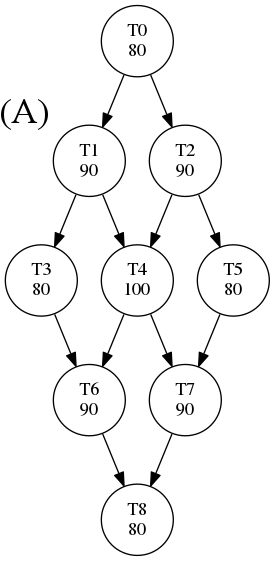
\includegraphics[width=0.21\textwidth]{laplace9a.png}}
  \subcaptionbox*{}{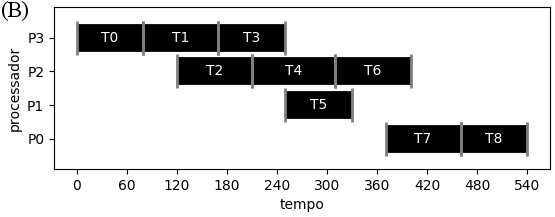
\includegraphics[width=0.70\textwidth]{ganttb.png}}
  \caption{ \textbf{(A)}: grafo laplace9 com custos de comunicação omitidos, que são iguais a 40 para todas as arestas. \textbf{(B)}: diagrama de Gantt que representa um possível escalonamento para 4 processadores com makespan de 540 unidades de tempo. }
   \label{fig:laplgantt}
\end{figure*}

O tempo do escalonamento ou \textit{makespan} corresponde ao ponto da linha do tempo em que a execução de todas as tarefas foi terminada. Isto corresponde à duração total do escalonamento. Um escalonamento ótimo é aquele que apresenta um \textit{makespan} mínimo.


\subsection{Algoritmo Genético}
Algoritmo Genético (AG) é uma meta-heurística proposta por John Holland que se inspira na evolução das espécies e tem sido usada para tratar diversos tipos de problemas relacionados a busca e otimização, incluindo o problema de escalonamento de tarefas \cite{Goldberg:1989:GAS:534133}.

Um AG opera de maneira estocástica para evoluir um conjunto de soluções com objetivo de encontrar uma solução globalmente satisfatória no espaço de busca de um problema. Para isso, deve ser definida uma forma de representação de uma solução e uma função para avaliação da mesma. Depois é escolhida um modo de inicializar uma população de soluções como ponto inicial da busca, os operadores que modificarão tal população iterativamente, e parâmetros numéricos que controlam seu comportamento. Tais componentes são detalhados a seguir.
% Além do problema de entrada, um AG possui uma série de parâmetros numéricos para controlar seu comportamento.


\textit{Representação genética} -- Dado um problema a ser resolvido pelo Algoritmo Genético, deve ser definida uma estrutura de dados que codifique uma solução pertencente ao espaço de busca do problema. Uma instância dessa estrutura de dados constitui um indivíduo (ou ``cromossomo'') que fará parte da população do AG. A representação genética clássica é um vetor binário. \cite{Goldberg:1989:GAS:534133}.

\textit{Fitness} -- Uma função de \textit{fitness} (aptidão) é escolhida para a avaliação da qualidade de um indivíduo. Em geral, todo indivíduo explorado pelo AG é avaliado.

\textit{População inicial} -- Gerar uma população inicial de indivíduos constitui a etapa de inicialização do AG. Dado um parâmetro \(N_{pop}\) que indica o tamanho da população, são gerados \(N_{pop}\) indivíduos, de forma estocástica, que representam soluções válidas e compõem a população a ser evoluída pelo algoritmo. Geralmente, a população de um AG é uma lista de indivíduos ordenada pelo \textit{fitness}. 

% A seguir, as operações genéticas que compõem a etapa iterativa do AG.

\textit{Seleção} -- A cada iteração (ou geração) do AG, pares de indivíduos são selecionados da população para serem recombinados, gerando novas soluções (filhos). Em geral, indivíduos são selecionados de acordo com seu \textit{fitness}, tal que indivíduos melhores terão maior probabilidade de se reproduzir. O número de pares a serem selecionados é obtido a partir da taxa de \textit{crossover} (\(T_{cross}\)), que é dada como parâmetro do AG. O método clássico para seleção é a roleta, que dá a cada indivíduo uma probabilidade de ser selecionado que é diretamente proporcional ao seu \textit{fitness} relativo aos demais indivíduos da população. \cite{Goldberg:1989:GAS:534133}


\textit{Crossover} -- O operador de \textit{crossover} é o método para gerar novos indivíduos a partir de um par de indivíduos pais. Seu objetivo é que os filhos possuam características de ambos os pais combinando suas representações. Por exemplo, \textit{crossover} de um ou mais pontos consiste em dividir dois indivíduos (representados por vetores) em várias secções delimitadas por pontos que são alternadamente permutadas para gerar dois filhos. \cite{Goldberg:1989:GAS:534133}


\textit{Mutação} -- Após o processo de \textit{crossover}, alguns dos indivíduos filhos podem sofrer uma modificação pelo operador de mutação. A probabilidade de haver mutação em um filho definida pela taxa de mutação (\(T_{mut}\)), a qual é dada como parâmetro do AG. Quando necessário, correções e adaptações são feitas para que o novo indivíduo represente uma solução válida, pertencente ao espaço de busca. Para a representação genética clássica de vetor binário, o método de mutação consiste em negar um de seus bits. \cite{Goldberg:1989:GAS:534133}


\textit{Reinserção} -- Dada uma lista de indivíduos pais e filhos, a operação de reinserção produz uma lista de indivíduos que constituirá a população na iteração seguinte combinando a população atual e a lista de filhos. \cite{Goldberg:1989:GAS:534133}


\subsection{Algoritmo Genético Multipopulação}

Um Algoritmo Genético paralelo é um modelo de AG para execução em sistemas multiprocessados visando obter um tempo de processamento menor em relação a execução serial. Segundo \citeauthor{cantu1998survey}, os vários tipos de AGs paralelos podem ser categorizados em:

\begin{itemize}
\item Paralelização global ou mestre-escravo: utiliza uma população única controlada por um programa mestre enquanto avaliações e/ou operadores genéticos são feitas por programas escravos.

\item Paralelização de fina granularidade: voltada para sistemas massivamente paralelos. Utiliza uma população única cujos indivíduos competem e reproduzem apenas com uma vizinhança limitada.

\item Paralelização multipopulação: utiliza várias populações semi-isoladas que se comunicam com uma certa frequência.
\end{itemize}

\citeauthor{Alba:1999:SPD:315491.315495} consideram AGs paralelos como uma classe distinta de meta-heurísticas por apresentarem a característica da interação local em subgrupos da população (com exceção da abordagem de paralelismo global), o que causa um impacto na qualidade das soluções. São citados casos em que AGs paralelos encontram soluções melhores do que as de AGs seriais. Os autores argumentam que a abordagem paralela é benéfica mesmo em sistemas que não possuam múltiplos processadores.

Algoritmo Genético multipopulação é a forma mais popular de AG paralelo \cite{cantu1998survey}. Um AGMP pode ser encarado como uma extensão da implementação de AG, em que vários AGs independentes são executados, trocando alguns indivíduos entre si ocasionalmente. Assim, é pode-se converter um AG serial em AGMP adicionando o procedimento de migração, e é possível executá-lo em vários tipos de sistemas diferentes, seja uma máquina com um número qualquer de processadores ou uma rede de computadores \cite{cantu1998survey}.

AGMP é também conhecido como: AG distribuído, por sua abordagem relacionada a paralelismo MIMD (múltiplas instruções, múltiplos dados); AG paralelo de grossa granularidade, por sua alta taxa de computação por comunicação; e AG baseado em ilhas, devido a sua semelhança com o modelo de ilhas em genética populacional. O AGMP se caracteriza por usar poucas populações de tamanho relativamente grande, em contraste com as pequenas e numerosas vizinhanças mantidas na abordagem de fina granularidade \cite{cantu1998survey}.

O funcionamento do AGMP também requer parâmetros adicionais como número de populações, frequência de migração (\(F_{mig}\)) e taxa de migração (\(T_{mig}\)). A seguir, são descritos os conceitos adicionais que caracterizem o AGMP.
% Abordagens para a comunicação entre populações de AGMP são apresentadas a seguir.

\textit{Topologia de comunicação} -- Estabelece as ligações entre populações, definindo as populações de destino a serem consideradas por cada população durante migrações. Topologias são geralmente especificadas \textit{a priori} e imutáveis ao longo da execução. \cite{cantu1998survey}


\textit{Frequência de migração} -- Define a periodicidade de trocas de indivíduos entre populações. Migrações podem ocorrer de modo síncrono num intervalo predeterminado de gerações, ou assíncrono sob satisfação de uma condição \cite{cantu1998survey}. Para o caso especial em que a frequência de migração é igual a zero, o AGMP é equivalente a uma sequência de execuções independentes de AG serial com população reduzida. Tal abordagem é desencorajada por \citeauthor{Cantu-Paz2003} por, geralmente, produzir soluções de baixa qualidade.


\textit{Seleção de migrantes} -- O critério de escolha de quais indivíduos serão removidos de sua população de origem para serem inseridos em outra. Em geral, imigrantes substituem indivíduos emigrantes ou os de pior \textit{fitness}. \cite{cantu1998survey}


\section{Trabalhos correlatos}

Trabalhos correlatos podem ser divididos entre aplicações de AG para o problema do escalonamento de tarefas e abordagens para desenvolvimento de AGMP de modo geral.

\subsection{Algoritmo Genético aplicado a escalonamento de tarefas}

 A maior parte dos trabalhos consultados formula suas representações considerando a ordenação topológica do grafo direcionado acíclico dado pelo problema de escalonamento, o que permite a disposição dos vértices em uma lista ordenada pela precedência. Assim, para toda aresta \(e_{ij}\), a posição da tarefa \(T_i\) na lista é anterior à posição de \(T_j\).

A representação genética de \citeauthor{Hou1994}, \citeauthor{Correa}, e \citeauthor{Kaur_heuristicsbased} mantém, para cada processador, uma lista de tarefas ordenada pela precedência. \citeauthor{WANG19978}, \citeauthor{OMARA201013}, \citeauthor{CHITRA20112725}, e \citeauthor{Morady} empregam dois vetores de inteiros: um representa uma ordenação topológica de tarefas e o outro representa o processador correspondente a cada tarefa. \citeauthor{Kwok:1997:ESA:274066.274077} utilizam uma única lista de tarefas ordenada por precedência, cujos processadores são atribuídos durante a computação do \textit{fitness}. \citeauthor{HWANG2008976} codificam a sequência de tarefas usando uma lista de prioridades numéricas, na qual os processadores associados correspondem ao valor da prioridade módulo o número de processadores. \citeauthor{XU2014255} fazem uso de uma fila de prioridade que indica a ordem de execução da tarefas.

Como função de \textit{fitness}, \citeauthor{Hou1994}, \citeauthor{WANG19978}, \citeauthor{Correa}, \citeauthor{HWANG2008976}, \citeauthor{OMARA201013}, \citeauthor{Morady} avaliam o \textit{makespan}. \citeauthor{Kwok:1997:ESA:274066.274077} usam o \textit{makespan} normalizado entre 0 e 1. \citeauthor{Kaur_heuristicsbased} consideram o \textit{makespan} e o ``\textit{flowtime}'', que foi definido como soma dos tempos de término de cada tarefa. \citeauthor{CHITRA20112725} fazem uma soma ponderada entre \textit{makespan} e confiabilidade, obtida ao contabilizar possíveis cenários de falha de processadores. \citeauthor{XU2014255} calculam o \textit{fitness} subtraindo o \textit{makespan} de um indivíduo do maior \textit{makespan} presente na população.

As populações iniciais de \citeauthor{Hou1994}, \citeauthor{Correa}, \citeauthor{HWANG2008976}, \citeauthor{CHITRA20112725}, \citeauthor{Morady} são formadas por indivíduos gerados aleatoriamente. \citeauthor{WANG19978}, \citeauthor{Kwok:1997:ESA:274066.274077}, \citeauthor{Kaur_heuristicsbased}, \citeauthor{OMARA201013}, \citeauthor{XU2014255} geram uma parte da população aleatoriamente e obtém a outra por heurísticas de ranqueamento de prioridade das tarefas.

Na literatura existem vários métodos para seleção. \citeauthor{Hou1994}, \citeauthor{WANG19978}, \citeauthor{HWANG2008976}, \citeauthor{Kaur_heuristicsbased}, \citeauthor{CHITRA20112725}, \citeauthor{XU2014255} utilizam o método da roleta, que associa a cada indivíduo uma probabilidade de ser selecionado diretamente relacionada a seu \textit{fitness}. \citeauthor{Kwok:1997:ESA:274066.274077} avaliam o \textit{fitness} de um indivíduo em relação ao \textit{fitness} médio da população para definir o número de vezes que cada indivíduo se reproduzirá. \citeauthor{OMARA201013} utilizam o método do torneio binário em que o melhor entre dois indivíduos selecionados aleatoriamente é escolhido. \citeauthor{Morady} fazem parte da seleção com torneio e parte com a escolha direta de uma porção dos melhores indivíduos da população.

Para \textit{crossover}, \citeauthor{WANG19978}, \citeauthor{Kwok:1997:ESA:274066.274077}, \citeauthor{CHITRA20112725}, \citeauthor{Kaur_heuristicsbased}, \citeauthor{OMARA201013}, \citeauthor{XU2014255} se baseiam em \textit{crossover} de um ponto, com estratégias para reordenar ou recombinar metade do cromossomo conforme necessário. \citeauthor{Hou1994} escolhem pontos de \textit{crossover} durante iterações sobre as listas de tarefas de cada processador. \citeauthor{Correa} aplicam \textit{crossover} uniforme: mantém-se as tarefas que coincidem nos pais e sorteia-se uma das alternativas caso contrário. \citeauthor{HWANG2008976} desenvolvem um método baseado em \textit{crossover} de dois pontos. \citeauthor{Morady} combinam \textit{crossover} de dois pontos e PMX, um algoritmo utilizado para vetores que envolvem permutação, que mantém uma subsequência do vetor inalterada e elimina elementos repetidos.

\textit{Swap} é o operador de mutação mais usado na literatura \cite{Hou1994,WANG19978,Kwok:1999:SSA:344588.344618,HWANG2008976,CHITRA20112725,XU2014255},
% \citeauthor{Hou1994}, \citeauthor{WANG19978}, \citeauthor{Kwok:1997:ESA:274066.274077}, \citeauthor{HWANG2008976}, \citeauthor{CHITRA20112725}, e \citeauthor{XU2014255} aplicam \textit{swap}
o qual consiste em trocar duas tarefas de lugar na sequência de execução, podendo implicar uma mudança de processador. O operador implementado por \citeauthor{OMARA201013} muda o processador em que uma tarefa é executada. \citeauthor{Correa} fazem a remoção de uma tarefa e sua reinserção num ponto diferente. \citeauthor{Kaur_heuristicsbased} e \citeauthor{Morady} usam duas operações: \textit{swap} sem mudança de processador ou apenas mudança de processador.

A reinserção nos trabalhos de \citeauthor{Hou1994}, \citeauthor{WANG19978}, \citeauthor{Kwok:1997:ESA:274066.274077}, \citeauthor{Correa}, \citeauthor{HWANG2008976}, \citeauthor{Kaur_heuristicsbased}, \citeauthor{CHITRA20112725}, \citeauthor{XU2014255}, e \citeauthor{Morady} é feita por elitismo: uma porção dos melhores indivíduos permanece na população e o restante é preenchido pelos filhos gerados.


\subsection{Abordagens em AGMP}
Os trabalhos \cite{Kwok:1997:ESA:274066.274077,Morady} apresentam aplicações de AGMP para escalonamento de tarefas. Os demais trabalhos consultados usam o AGMP para outras aplicações: escalonamento job-shop \cite{Qi2000}, \textit{data mining} \cite{Srinivasa:2007:SMM:1279013.1279229}, carregamento de contêiners \cite{Gehring}, otimização de funções \cite{Muhlenbein:1991:PPG:1746086.1746158,Yao}, e otimização combinatória \cite{Han}.
%  O trabalho de \citeauthor{Morady} foi o único encontrado que apresenta uma aplicação de AGMP para escalonamento de tarefas com custos de comunicação.

A respeito de topologia de comunicação, as populações de \citeauthor{Kwok:1997:ESA:274066.274077}, \citeauthor{Qi2000}, e \citeauthor{Srinivasa:2007:SMM:1279013.1279229} são totalmente conectadas. \citeauthor{Gehring} e \citeauthor{Morady} usam topologia em anel, na qual cada população possui uma única população de destino, descrevendo um anel conectado. \citeauthor{Muhlenbein:1991:PPG:1746086.1746158} dispõem uma estrutura de ``escada circular'', com múltiplas conexões em cada população. \citeauthor{Han} aplicam, uma estrutura de agrupamento voltada para a redução da carga de comunicação entre processadores. \citeauthor{Yao} utilizam uma topologia dinâmica em que populações podem se unir ou dividir durante a execução.

A frequência de migração é um parâmetro fixo nos trabalhos \cite{Muhlenbein:1991:PPG:1746086.1746158,Qi2000,Han,Gehring,Srinivasa:2007:SMM:1279013.1279229,Morady}, enquanto 
% \cite{Muhlenbein:1991:PPG:1746086.1746158}, \cite{Qi2000}, \cite{Han}, \cite{Gehring}, \cite{Srinivasa:2007:SMM:1279013.1279229}, \cite{Morady}. 
\citeauthor{Kwok:1997:ESA:274066.274077} empregam uma frequência exponencialmente crescente ao longo da execução.

Em \cite{Muhlenbein:1991:PPG:1746086.1746158,Kwok:1997:ESA:274066.274077,Qi2000,Han,Gehring,Srinivasa:2007:SMM:1279013.1279229,Morady},
% \cite{Muhlenbein:1991:PPG:1746086.1746158}, \cite{Kwok:1997:ESA:274066.274077}, \cite{Qi2000}, \cite{Han}, \cite{Gehring}, \cite{Srinivasa:2007:SMM:1279013.1279229}, e \cite{Morady},
os melhores indivíduos são selecionados para migração. Migrações são determinadas por meio de uma análise de agrupamento de indivíduos em~\cite{Yao}. 


\section{Desenvolvimento}

O trabalho desenvolvido consistiu em quatro etapas: selecionar um conjunto de grafos para \textit{benchmark}, a ser utilizado nas avaliações comparativas dos algoritmos implementados; implementar o AG e suas diferentes configurações de \textit{crossover}; implementar o AGMP; comparar as melhores configurações do AG e do AGMP.

\subsection{Grafos para \textit{benchmark}}
\label{sec:grafos}
Para fins de comparação, foi elaborado um conjunto de grafos referentes ao problema de escalonamento com custos de comunicação em algoritmos reais.

%, uma vez que não foi encontrada uma base de dados padronizada como \textit{benchmark}.

Compondo esse conjunto, foram utilizados grafos obtidos diretamente de outros trabalhos e também famílias de grafos baseadas em instâncias usadas na literatura.


\subsubsection{Grafos relacionados a problemas paralelos reais}

Com o objetivo de incrementar o conjunto com grafos relevantes e com espaços de busca de alta cardinalidade, foram implementados três scripts em linguagem Python que geram grafos pertencentes a ``famílias'' correspondentes a algoritmos paralelos mencionados na literatura: eliminação gaussiana, algoritmo de Laplace e transformada rápida de Fourier \cite{olteanu}. Assim, um grafo pertencente a uma dessas famílias corresponde à execução do algoritmo para um dado tamanho de entrada. A metodologia adotada na  geração desses grafos foi inspirada no trabalho descrito em \cite{olteanu}.

Os scripts implementados geram representações de grafos em arquivos de texto e também suas visualizações com a ferramenta Graphviz. Quatro grafos de cada família foram selecionados para compor o conjunto de \textit{benchmark}, num total de 12 grafos baseados em programas paralelos reais.

A família ``gauss'' é definida pelo algoritmo da Decomposição LU, uma forma matricial do método da eliminação gaussiana. Esse algoritmo que realiza fatoração de matrizes quadradas em matrizes triangulares, o que se reflete na estrutura desses grafos. Seu número de tarefas depende diretamente do tamanho da matriz de entrada, e seus pesos e custos de comunicação obedecem um padrão regular \cite{jiang}. A Figura \ref{fig:gauss} mostra duas instâncias desta família, nas quais as arestas contínuas representam custo de comunicação igual a $12$ e as arestas tracejadas, custo igual a $8$ \cite{COSNARD1988275}.


\begin{figure*}
  \centering
  \subcaptionbox*{}{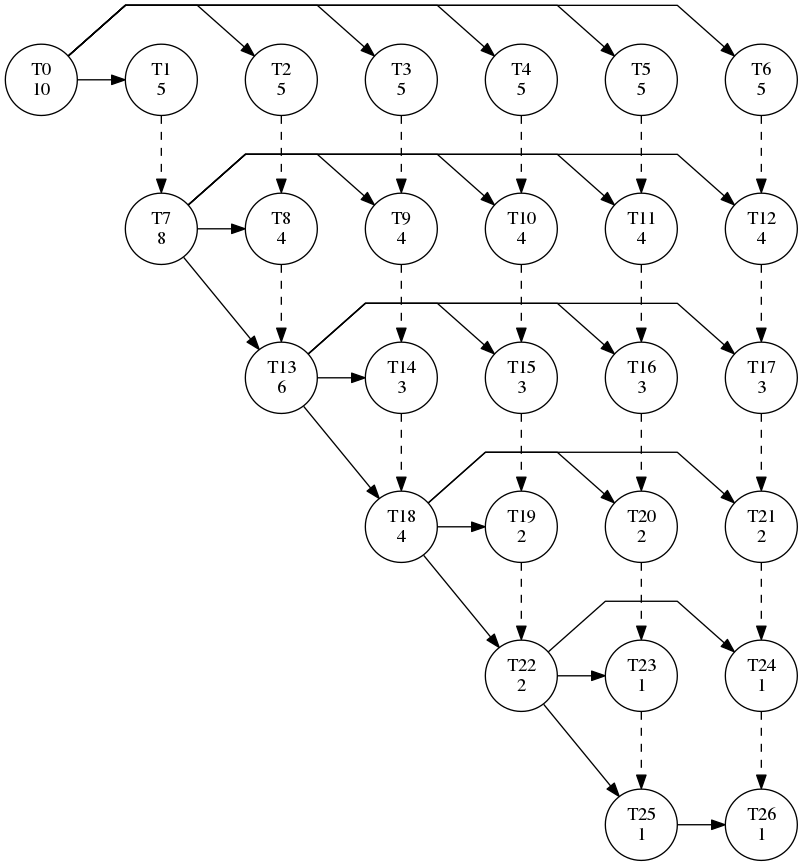
\includegraphics[width=0.40\textwidth,valign=b]{gauss27.png}} 
  \subcaptionbox*{}{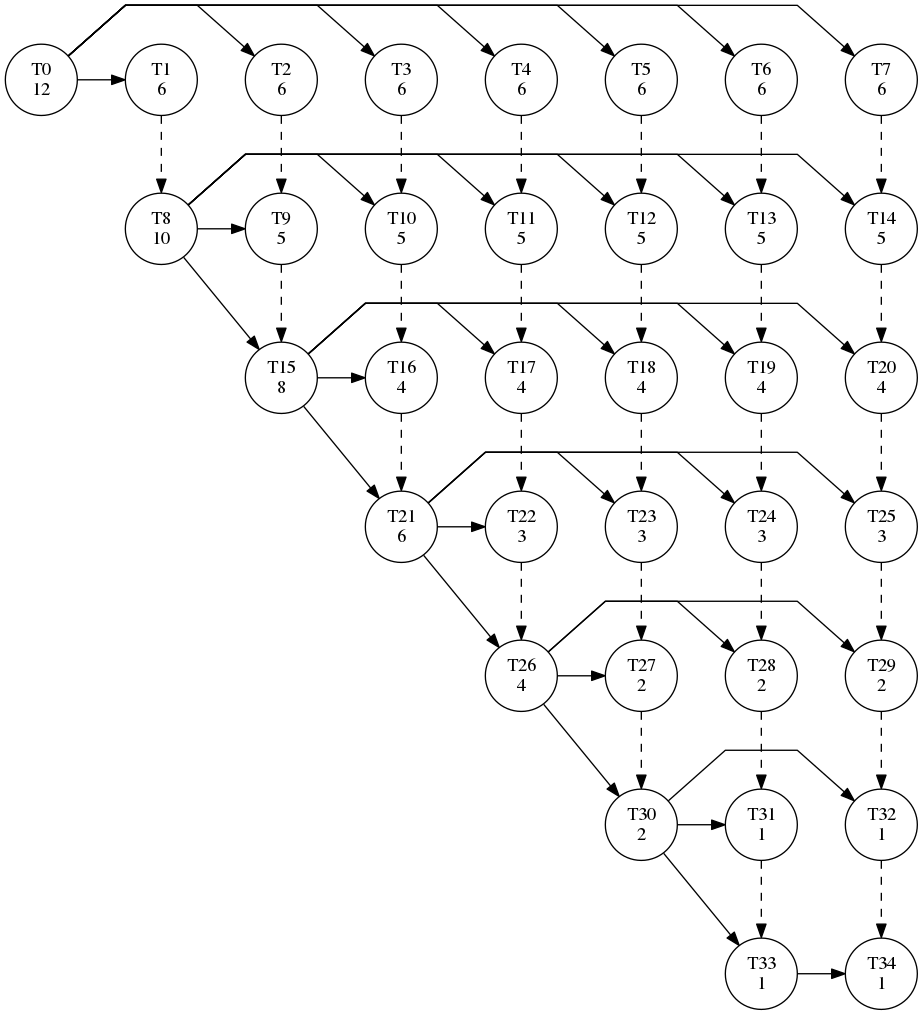
\includegraphics[width=0.46\textwidth,valign=b]{gauss35.png}}
  \caption{Grafos gauss27 e gauss35. Arestas contínuas representam custo de comunicação igual a 12 e arestas tracejadas, custo igual a 8. Fonte: elaborada pelos autores.}
   \label{fig:gauss}
\end{figure*}

\begin{figure*}
  \centering
  \subcaptionbox*{}{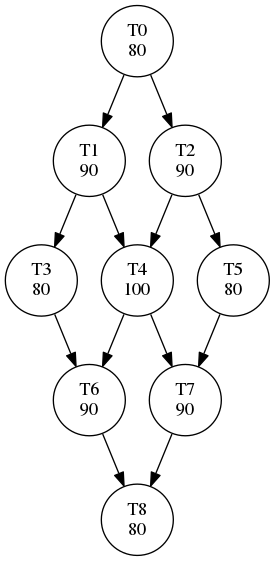
\includegraphics[width=0.20\textwidth,valign=c]{laplace9.png}} 
  \subcaptionbox*{}{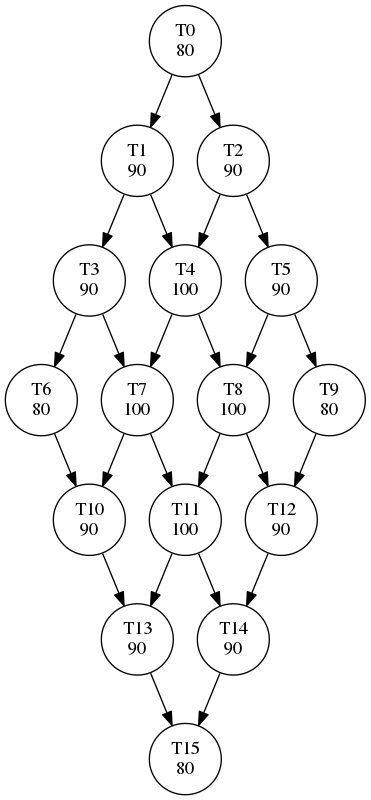
\includegraphics[width=0.28\textwidth,valign=c]{laplace16.png}}
  \caption{Grafos laplace9 e laplace16. Todos os custos de comunicação nesta família são iguais a 40. Fonte: elaborada pelos autores.}
  \label{fig:laplace}
\end{figure*}

\begin{figure*}
  \centering
  \subcaptionbox*{}{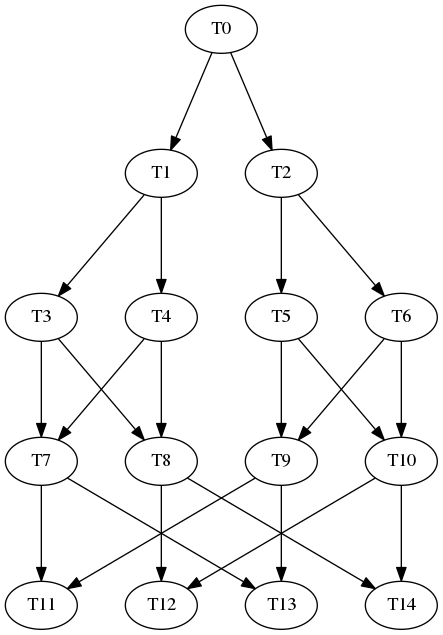
\includegraphics[width=0.28\textwidth,valign=c]{fft15.png}} 
  \subcaptionbox*{}{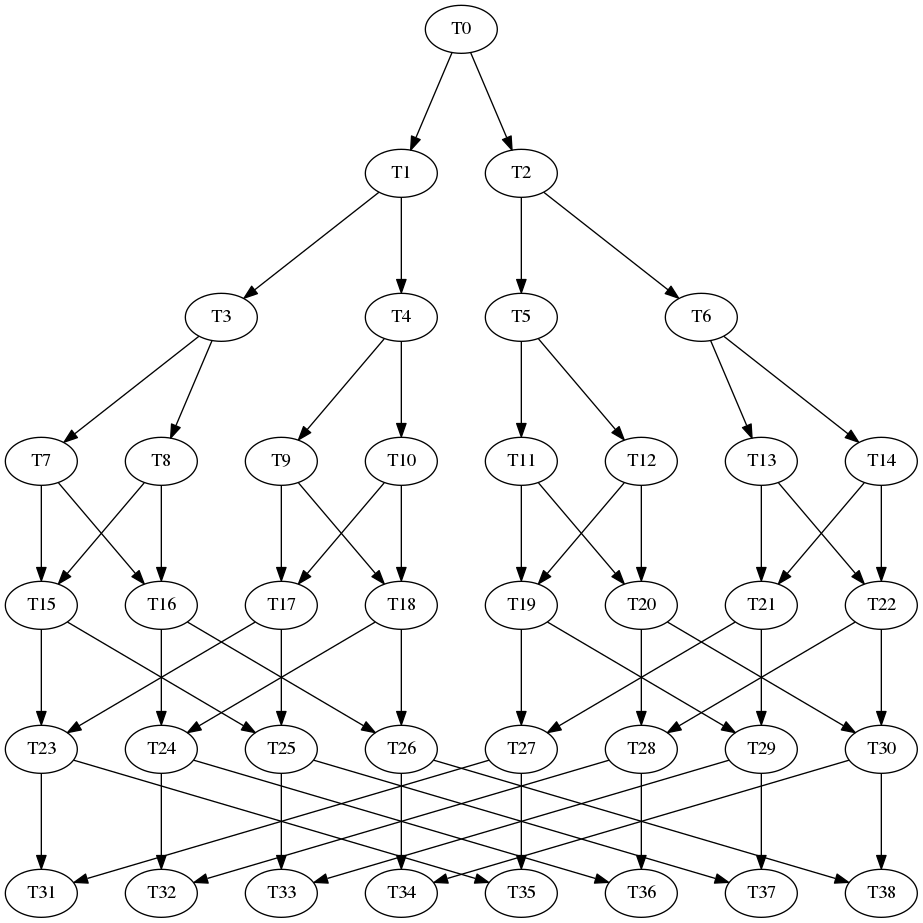
\includegraphics[width=0.58\textwidth,valign=c]{fft39.png}}
  \caption{Grafos fft15 e fft39. Nesta família, os vértices  possuem pesos iguais a 60 e os custos de comunicação são iguais a 80. Fonte: elaborada pelos autores.}
  \label{fig:fft}
\end{figure*}


A família ``laplace'' é dada pelo algoritmo para resolução de equações de Laplace, composta por uma estrutura de tarefas que reflete diretamente o seu tamanho de entrada, que é uma matriz quadrada. Nesta família, ilustrada na Figura \ref{fig:laplace}, as dependências entre tarefas são dadas pela maneira em que a matriz é percorrida no algoritmo \cite{hypertool}. Nesta família, os pesos das tarefas obedecem um padrão regular e todos os custos de comunicação são iguais a 40. Os pesos de cada tarefa correspondem à posição do elemento correspondente na matriz, sendo $80$ para as tarefas nas 4 extremidades do grafo (acima, abaixo, à direita e à esquerda), $90$ para as tarefas nas laterais, e $100$ para as tarefas mais internas.



A família ``fft'' é baseada no algoritmo de Cooley–Tukey para a transformada rápida de Fourier. Esta família de grafos assume como entrada uma lista de tamanho igual a uma potência de 2. Seus grafos assumem uma estrutura com uma etapa recursiva e uma etapa de operação ``borboleta'' característica do algoritmo \cite{fft}. Duas instâncias são mostradas na Figura \ref{fig:fft}. Os pesos e custos de comunicação nesta família são iguais a 60 e 80, respectivamente.


\subsubsection{Outros grafos}

Em \cite{Morady} foram disponibilizados onze grafos com número de vértices entre 4 e 18, obtidos de diversos trabalhos da literatura. Aqui, eles são referenciados com prefixo ``TG''. Os autores não mencionam correspondência entre esses grafos e algoritmos paralelos reais.

Em \cite{murillo} foi utilizada uma ferramenta para criação de três grafos aleatórios com 30, 40 e 50 vértices, identificados pelo prefixo ``random''.

No total, o conjunto do \textit{benchmark} é composto por 26 grafos, sendo 12 gerados a partir de informações de programas paralelos reais e 14 extraídos da literatura sem conexão com problemas reais.


\subsection{Algoritmo Genético Serial}

O primeiro algoritmo evolutivo construído foi um AG serial para o problema do escalonamento de tarefas. Nessa etapa, algumas configurações relevantes do AG foram definidas e comparadas a fim de obter uma boa opção de operadores e parâmetros. O propósito deste trabalho foi explorar abordagens de AG ``puro'', em contraste com a tendência recente de desenvolver AGs híbridos incorporando diversas técnicas e heurísticas específicas do problema \cite{Kaur_heuristicsbased,WANG19978,OMARA201013,XU2014255,Kwok:1997:ESA:274066.274077}.

A representação do indivíduo utilizada é a mesma de \cite{WANG19978}, \cite{OMARA201013}, \cite{CHITRA20112725}, e \cite{Morady}: dois vetores de inteiros \(S,P\) tal que \(S\) é uma sequência de tarefas que obedece às restrições de ordenação topológica do grafo dado e \(P\) é um vetor que mapeia os vínculos tarefa/processador de forma que \(P[tarefa] = processador\).



A Figura \ref{fig:repr}B ilustra um indivíduo válido para o grafo laplace9 (Figura \ref{fig:repr}A), considerando-se alocação para 4 processadores. Para representar seu escalonamento correspondente, ilustrado na Figura \ref{fig:repr}C, o vetor \(S = [0,2,5,1,3,4,6,7,8]\) é particionado em uma sequência para cada processador, obedecendo as associações dadas pelo vetor \(P = [3,3,2,3,2,1,2,0,0]\). Por exemplo, as tarefas executadas pelo processador P3 são T0, T1 e T3, pois \(P[0] = P[1] = P[3] = 3\). O processamento de cada tarefa é iniciado após a conclusão de todas as suas predecessoras, somado ao custo de comunicação em caso de serem executadas em processadores diferentes. Por exemplo, a tarefa T5 é iniciada após a conclusão e comunicação de T2. Com isso, T5 é executada após o início de T4, embora T5 seja anterior a T4 no vetor \(S\).


\begin{figure*}
  \centering
  \subcaptionbox*{}{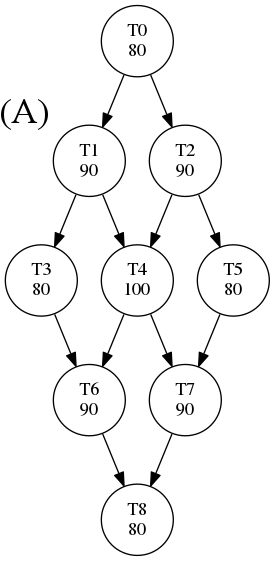
\includegraphics[width=0.21\textwidth,valign=c]{laplace9a.png}} 
  \subcaptionbox*{}{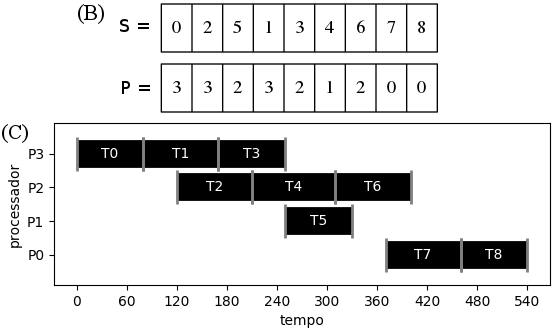
\includegraphics[width=0.70\textwidth,valign=c]{gantt2.png}}
  \caption{ \textbf{(A)}: grafo laplace9 com custos de comunicação omitidos, que são iguais a 40 para todas as arestas.
  \textbf{(B)}: exemplo de indivíduo para o grafo laplace9 e 4 processadores.
  \textbf{(C)}: diagrama de Gantt que representa o escalonamento correspondente ao indivíduo de (B), com \textit{makespan} de 540 unidades de tempo.}
  \label{fig:repr}
\end{figure*}


A função de \textit{fitness} utilizada é dada pelo \textit{makespan} associado ao escalonamento. Por exemplo, o indivíduo representado na Figura \ref{fig:repr}B tem \textit{fitness} igual a 540, que corresponde ao tempo de finalização do processador P0, o mais tardio na Figura 5C. A população inicial é gerada aleatoriamente com indivíduos válidos: vetor \(S\) sem repetição das tarefas e respeitando as restrições de ordenação topológica. A seleção dos pais para o \textit{crossover} é feita com torneio binário. A reinserção da população no final de cada geração se dá por elitismo. A mutação é uma operação pontual em um dos dois vetores do indivíduo, mudando o processador de uma tarefa ou trocando duas tarefas de lugar na sequência caso não haja dependência entre elas. Essas duas operações de mutação são referidas aqui como mutação ``proc'' e mutação ``seq'', respectivamente.

Como a representação adotada é formada por duas partes distintas (\(S\) e \(P\)), existe uma variedade de opções diferentes para a aplicação do operador de \textit{crossover}. Três abordagens foram observadas na bibliografia, aqui nomeadas como \textit{carry}, \textit{choose} e \textit{combine}:

\begin{itemize}
\item{\textit{Carry}}: o \textit{crossover} é aplicado no vetor de tarefas ``carregando'' o vínculo de cada tarefa com o processador definido no pai correspondente. Assim, tarefas do indivíduo filho vindas do pai1 possuem o mesmo processador do pai1. Do mesmo modo, tarefas vindas do pai2 são executadas nos processadores definidos no pai2. Esta abordagem é análoga a métodos usados em trabalhos com representação de listas de tarefas por processador \cite{Hou1994}, \cite{Correa}, \cite{Kaur_heuristicsbased}.

\item{\textit{Choose}}: é definida uma operação de \textit{crossover} para o vetor de tarefas e uma para o vetor de processadores. Durante a reprodução de indivíduos, um dos dois tipos de \textit{crossover} é sorteado e aplicado. O outro vetor é copiado do primeiro pai para o primeiro filho e vice-versa \cite{OMARA201013}.

\item{\textit{Combine}}: é definido um \textit{crossover} para o vetor de tarefas e um para o vetor de processadores. Durante a reprodução de indivíduos, ambos \textit{crossovers} são aplicados \cite{Morady}.
\end{itemize}

Para avaliar estes métodos, foram implementados os seguintes algoritmos clássicos de \textit{crossover}, que foram adaptados para evitar duplicação de tarefas e obedecer as restrições do vetor de tarefas ($S$):

\begin{itemize}
\item 1-ponto: sorteia-se um ponto de corte na sequência. Copia-se a primeira parte do pai1 e a segunda parte é preenchida, sem repetição, com tarefas seguindo a ordem em que se elas estão dispostas no pai2 \cite{OMARA201013}.

\item 2-pontos: análogo ao anterior; a sequência é dividida em 3 partes. A primeira é uma cópia do pai1, a segunda é preenchida com tarefas na ordem do pai2, e a terceira é preenchida com tarefas restantes do pai1, também obedecendo sua ordem.

\item Uniforme: a sequência filha é composta percorrendo os pais e escolhendo aleatoriamente de qual pai será herdada a tarefa seguinte, ignorando repetições.

\item Cíclico: uma posição p é sorteada e os p-ésimos elementos das sequências são trocados. Enquanto houver uma duplicata na primeira sequência, o elemento repetido é trocado pelo elemento na mesma posição na outra sequência. É necessária validação posterior para garantir as restrições de precedência.

\item PMX: mantém-se uma subsequência do pai1, troca-se o restante com elementos do pai2 e faz-se trocas até eliminar duplicatas. Também é necessária validação do filho.

\item OX: mantém-se uma subsequência do pai1 e preenche-se o restante seguindo a ordem do pai2. A versão implementada gera um filho válido por garantir que todas as tarefas predecessoras da subsequência estejam à esquerda dela.
\end{itemize}

Alguns desses métodos de \textit{crossover} são exemplificados para o grafo laplace9 na Figura \ref{fig:cross}, em que filhos $F1$, $F2$, $F3$ e $F4$ foram produzidos respectivamente por \textit{crossover} 1-ponto, 2-pontos, uniforme, OX, a partir dos pais $P1$ e $P2$. Além deles, foram implementados \textit{crossovers} 1-ponto, 2-pontos e uniforme para o vetor de processadores, que são análogos aos descritos e sem restrição sobre repetição e ordenação. A implementação foi feita em linguagem C e compilada e otimizada com GCC. Os resultados dos experimentos com o algoritmo evolutivo serial serão apresentados na Seção 5.

\begin{figure*}
  \centering
  \subcaptionbox*{}{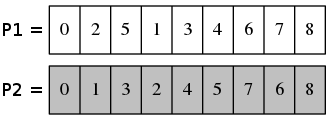
\includegraphics[width=0.4\textwidth,valign=t]{parents.png}} \hspace{0.1\textwidth}
  \subcaptionbox*{}{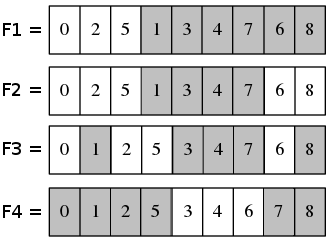
\includegraphics[width=0.4\textwidth,valign=t]{children.png}}
  \caption{ Exemplos de \textit{crossover} sobre vetores de tarefa para o grafo laplace9, omitindo vetores de processadores ($P$) dos indivíduos. À esquerda, as tarefas dos indivíduos pais. À direita, tarefas de filhos gerados por \textit{crossovers} 1-point ($F1$), 2-point ($F2$), uniforme ($F3$) e OX ($F4$). }
  \label{fig:cross}
\end{figure*}


\subsection{Algoritmo Genético Multipopulação}

O AGMP desenvolvido nesse trabalho emprega topologia em anel unidirecional para comunicação entre as populações, que é um modelo de simples implementação e que produziu resultados de boa qualidade em trabalhos correlatos \cite{cantu1998survey}. No anel unidirecional, toda população tem uma vizinha para onde envia alguns indivíduos, e uma segunda vizinha da qual recebe outros indivíduos em um processo conhecido por migração. Os melhores indivíduos da população são os selecionados para a migração. Os parâmetros de migração foram definidos experimentalmente: \(T_{mig} = 10\%\) e \(F_{mig} = 5\). Demais parâmetros são dados pela \textit{config6} (Tabela \ref{tab:configs}), escolhida para o AG serial.

Note que a quantidade de avaliações de \textit{fitness} realizadas pelo AGMP é igual à do AG, pois o número total de indivíduos é distribuído igualmente entre cada população. Por exemplo, para 400 indivíduos e 4 populações, o tamanho de cada uma é igual a 100.

A taxa de migração é relativa ao tamanho das populações. No exemplo de 4 populações com 100 indivíduos cada, os parâmetros de migração ditam que os 10 melhores indivíduos (10\%) de cada população migrarão.

A implementação foi feita estendendo o AG com procedimentos de inicialização das populações e migração, que foram feitos em memória distribuída com a biblioteca OpenMPI, que implementa o padrão \textit{Message Passing Interface} para execução paralela de programas com múltiplos processos. Desse modo, cada população é executada em um processo diferente que se comunica com populações vizinhas de acordo com a frequência de migração. Por fim, os melhores indivíduos de cada população são enviados para uma mesma população, e o melhor deles é retornado pelo programa. Os demais operadores (seleção, \textit{crossover}, mutação e reinserção) foram implementados  da mesma forma descrita para o AG Serial na seção anterior. Uma execução do AG serial é equivalente a executar o AGMP com número de populações igual a 1.

\section{Experimentos e Resultados}

Nesta seção são definidos os parâmetros utilizados nos algoritmos evolutivos e o método adotado nos experimentos. Em seguida, o AG e o AGMP são comparados em termos de qualidade das soluções produzidas e tempo de execução.

\subsection{Definições iniciais de parâmetros e configurações}
\label{sec:param}

Para escolha do método de aplicação de \textit{crossover}, foram elaboradas execuções do AG serial com configurações baseadas na literatura, apresentadas na Tabela \ref{tab:configs}, que contém duplas de operações de \textit{crossover} para vetor de tarefas e de processadores em casos do tipo \textit{choose} ou \textit{combine} e apenas um tipo de \textit{crossover} para o vetor de tarefas no caso \textit{carry}.

\textit{Config0} é uma configuração sugerida nas fases iniciais deste trabalho a partir de experiências anteriores do grupo com o problema. \textit{Config1} é baseada na descrição de \citeauthor{OMARA201013}. \textit{Config2} é igual à anterior, com a adição de mutação no vetor de tarefas (mutação ``seq''). \textit{Config3} é baseada em \cite{Correa}, com a representação genética de dois vetores aqui descrita em vez de listas de tarefas para cada processador. \textit{Config4} é igual à anterior com seleção via torneio em vez de roleta. \textit{Config12} segue o trabalho de \citeauthor{Morady}. As restantes são algumas variações das configurações anteriores.

\begin{table}[h]
\footnotesize
\centering
\caption{Configurações de AG}
\begin{tabular}{|l|l|l|l|l|}
\hline
\textbf{config} & \textbf{seleção}  & \textbf{método}  & \textbf{\textit{crossover}}       & \textbf{mutação}  \\ \hline
0      & torneio  & \textit{carry}   & cíclico            & seq/proc \\ \hline
1      & torneio  & \textit{choose}  & 1-point, 1-point   & proc     \\ \hline
2      & torneio  & \textit{choose}  & 1-point, 1-point   & seq/proc \\ \hline
3      & roleta   & \textit{carry}   & uniforme           & seq/proc \\ \hline
4      & torneio  & \textit{carry}   & uniforme           & seq/proc \\ \hline
5      & torneio  & \textit{choose}  & 2-point, 2-point   & seq/proc \\ \hline
6      & torneio  & \textit{combine} & 1-point, 1-point   & seq/proc \\ \hline
7      & torneio  & \textit{combine} & uniforme, uniforme & seq/proc \\ \hline
8      & torneio  & \textit{combine} & 2-point, 2-point   & seq/proc \\ \hline
9      & torneio  & \textit{choose}  & uniforme, uniforme & seq/proc \\ \hline
10     & torneio  & \textit{carry}   & pmx                & seq/proc \\ \hline
11     & torneio  & \textit{carry}   & ox                 & seq/proc \\ \hline
12     & torneio  & \textit{combine} & pmx, 2-point       & seq/proc \\ \hline
13     & torneio  & \textit{combine} & cíclico, 2-point   & seq/proc \\ \hline
14     & torneio  & \textit{combine} & ox, 2-point        & seq/proc \\ \hline
\end{tabular}
\label{tab:configs}
\end{table}

O número de avaliações de \textit{fitness} feitas em uma execução do AG representa o número aproximado de pontos explorados no espaço de busca. Esse número decorre dos parâmetros adotados no AG, e pode conter imprecisão devido à possibilidade da avaliação de um indivíduo repetido. Os parâmetros usados por \citeauthor{Morady} foram tomados como ponto de partida neste trabalho: $N_{pop} = 200$, $N_{ger} = 400$, $T_{cross} = 65\%$ e $T_{mut} = 35\%$. Desse modo, os parâmetros iniciais totalizam 52.200 avaliações de \textit{fitness}, de acordo com o cálculo a seguir, baseado na atual implementação:
\[avaliacoes = N_{pop} + N_{ger} * N_{pop} * T_{cross}\]
\[ avaliacoes = 200 + 400 * 200 * 0,65 = 52.200\]

Porém, foi observado que as configurações implementadas produziam resultados melhores se a população fosse maior em relação ao número de gerações ($N_{ger}$). Então, os parâmetros adotados foram: $N_{pop} = 400$, $N_{ger} = 198$, $T_{cross} = 65\%$ e $T_{mut} = 35\%$, totalizando 51.880 avaliações de \textit{fitness}, ou seja, aproximadamente o mesmo número de avaliações adotado em \cite{Morady}.

\subsection{Metodologia}

Para avaliar a qualidade das soluções de cada configuração e levando-se em conta o comportamento estocástico dos AGs, os experimentos consistem em 100 execuções para cada grafo do conjunto de \textit{benchmark} em cada uma das configurações da Tabela \ref{tab:configs}. Os dados avaliados incluem: convergência (número de vezes em que foi encontrada uma solução ótima); melhor \textit{fitness} obtido; \textit{fitness} médio; pior \textit{fitness}.

Entretanto, as soluções ótimas não são conhecidas para a maioria dos grafos do \textit{benchmark} elaborado, que foi descrito na Seção \ref{sec:grafos}. Desse modo, os melhores \textit{fitness} encontrados nos experimentos foram tomados como valores pseudo-ótimos, que são suficientes para realizar os experimentos comparativos. Estes valores são apresentados na Tabela \ref{tab:opt}.

%Desse modo, os valores ótimos de cada grafo foram estimados através de algumas execuções dos algoritmos usando parâmetros mais robustos que totalizaram mais de 600.000 pontos de busca em cada execução. Foram realizadas  100 execuções do AG robusto com uma população de 1200 indivíduos e 800 gerações. Os menores valores de \textit{makespan} obtidos nas 100 execuções para cada grafo e número de processadores, são apresentados na Tabela \ref{tab:opt}. Esses resultados foram considerados como ``ótimos'' no presente trabalho.
 
% \textbf{É possível observar que nem sempre o aumento de processadores na arquitetura acarreta numa diminuição do \textit{makespan}. Isso foi particularmente observado no aumento de 8 para 16 processadores. Acreditamos que na maioria dos casos, essa manutenção do valor ótimo (quando o número de processadores é duplicado) ocorre devido ao fato de que a estrutura do programa paralelo de fato não se beneficia do número elevado de processadores. Entretanto, devemos ter em mente que mesmo que a mudança da arquitetura não altere o ótimo, o espaço de busca é aumentado significativamente e a convergência do AG para ótimo torna-se bem mais difícil. Uma prova disso é que nos experimentos com os AGs com parâmetros mais limitados, similares ao número de avaliações efetuado em \cite{Morady}, tivemos diversas situações em que o melhor \textit{makespan} foi diminuído com a duplicação do número de processadores. Desse modo, embora não possamos assegurar que os valores da Tabela \ref{tab:opt} são de fato os ótimos globais, consideramos os mesmos bons o suficiente para serem utilizados como referência em nosso experimentos.}

% \begin{table}
% \centering
% \caption{Valores estimados de \textit{fitness} ótimos.}
% \label{tab:opt}
% \begin{tabular}{lllll}
% \cline{2-5}
% & \multicolumn{4}{|c|}{\textbf{número de processadores}} \\
%  \hline
% \multicolumn{1}{|l|}{\textbf{grafo}}     & \multicolumn{1}{l|}{\textbf{2}}    & \multicolumn{1}{l|}{\textbf{4}}    & \multicolumn{1}{l|}{\textbf{8}}    & \multicolumn{1}{l|}{\textbf{16}}   \\ \hline
% \multicolumn{1}{|l|}{TG4}       & \multicolumn{1}{l|}{34}   & \multicolumn{1}{l|}{34}   & \multicolumn{1}{l|}{34}   & \multicolumn{1}{l|}{34}   \\ \hline
% \multicolumn{1}{|l|}{TG9}       & \multicolumn{1}{l|}{21}   & \multicolumn{1}{l|}{21}   & \multicolumn{1}{l|}{21}   & \multicolumn{1}{l|}{21}   \\ \hline
% \multicolumn{1}{|l|}{TG10}      & \multicolumn{1}{l|}{97}   & \multicolumn{1}{l|}{83}   & \multicolumn{1}{l|}{83}   & \multicolumn{1}{l|}{83}   \\ \hline
% \multicolumn{1}{|l|}{TG11}      & \multicolumn{1}{l|}{22}   & \multicolumn{1}{l|}{20}   & \multicolumn{1}{l|}{20}   & \multicolumn{1}{l|}{20}   \\ \hline
% \multicolumn{1}{|l|}{TG12}      & \multicolumn{1}{l|}{27}   & \multicolumn{1}{l|}{27}   & \multicolumn{1}{l|}{27}   & \multicolumn{1}{l|}{27}   \\ \hline
% \multicolumn{1}{|l|}{TG14}      & \multicolumn{1}{l|}{35}   & \multicolumn{1}{l|}{35}   & \multicolumn{1}{l|}{35}   & \multicolumn{1}{l|}{35}   \\ \hline
% \multicolumn{1}{|l|}{TG17}      & \multicolumn{1}{l|}{41}   & \multicolumn{1}{l|}{37}   & \multicolumn{1}{l|}{36}   & \multicolumn{1}{l|}{36}   \\ \hline
% \multicolumn{1}{|l|}{TG18}      & \multicolumn{1}{l|}{440}  & \multicolumn{1}{l|}{440}  & \multicolumn{1}{l|}{440}  & \multicolumn{1}{l|}{440}  \\ \hline
% \multicolumn{1}{|l|}{TGb9}      & \multicolumn{1}{l|}{17}   & \multicolumn{1}{l|}{16}   & \multicolumn{1}{l|}{16}   & \multicolumn{1}{l|}{16}   \\ \hline
% \multicolumn{1}{|l|}{TGb11}     & \multicolumn{1}{l|}{49}   & \multicolumn{1}{l|}{49}   & \multicolumn{1}{l|}{49}   & \multicolumn{1}{l|}{49}   \\ \hline
% \multicolumn{1}{|l|}{TGc11}     & \multicolumn{1}{l|}{15}   & \multicolumn{1}{l|}{12}   & \multicolumn{1}{l|}{12}   & \multicolumn{1}{l|}{12}   \\ \hline
% \multicolumn{1}{|l|}{gauss27}   & \multicolumn{1}{l|}{69}   & \multicolumn{1}{l|}{67}   & \multicolumn{1}{l|}{67}   & \multicolumn{1}{l|}{67}   \\ \hline
% \multicolumn{1}{|l|}{gauss35}   & \multicolumn{1}{l|}{96}   & \multicolumn{1}{l|}{91}   & \multicolumn{1}{l|}{91}   & \multicolumn{1}{l|}{91}   \\ \hline
% \multicolumn{1}{|l|}{gauss44}   & \multicolumn{1}{l|}{132}  & \multicolumn{1}{l|}{116}  & \multicolumn{1}{l|}{116}  & \multicolumn{1}{l|}{116}  \\ \hline
% \multicolumn{1}{|l|}{gauss65}   & \multicolumn{1}{l|}{233}  & \multicolumn{1}{l|}{173}  & \multicolumn{1}{l|}{173}  & \multicolumn{1}{l|}{173}  \\ \hline
% \multicolumn{1}{|l|}{laplace9}  & \multicolumn{1}{l|}{520}  & \multicolumn{1}{l|}{520}  & \multicolumn{1}{l|}{520}  & \multicolumn{1}{l|}{520}  \\ \hline
% \multicolumn{1}{|l|}{laplace16} & \multicolumn{1}{l|}{840}  & \multicolumn{1}{l|}{760}  & \multicolumn{1}{l|}{760}  & \multicolumn{1}{l|}{760}  \\ \hline
% \multicolumn{1}{|l|}{laplace25} & \multicolumn{1}{l|}{1270} & \multicolumn{1}{l|}{1000} & \multicolumn{1}{l|}{1000} & \multicolumn{1}{l|}{1000} \\ \hline
% \multicolumn{1}{|l|}{laplace36} & \multicolumn{1}{l|}{1800} & \multicolumn{1}{l|}{1260} & \multicolumn{1}{l|}{1240} & \multicolumn{1}{l|}{1240} \\ \hline
% \multicolumn{1}{|l|}{fft15}     & \multicolumn{1}{l|}{580}  & \multicolumn{1}{l|}{560}  & \multicolumn{1}{l|}{560}  & \multicolumn{1}{l|}{560}  \\ \hline
% \multicolumn{1}{|l|}{fft39}     & \multicolumn{1}{l|}{1260} & \multicolumn{1}{l|}{820}  & \multicolumn{1}{l|}{800}  & \multicolumn{1}{l|}{800}  \\ \hline
% \multicolumn{1}{|l|}{fft95}     & \multicolumn{1}{l|}{2940} & \multicolumn{1}{l|}{1600} & \multicolumn{1}{l|}{1160} & \multicolumn{1}{l|}{1140} \\ \hline
% \multicolumn{1}{|l|}{fft223}    & \multicolumn{1}{l|}{6780} & \multicolumn{1}{l|}{3520} & \multicolumn{1}{l|}{2060} & \multicolumn{1}{l|}{1560} \\ \hline
% \multicolumn{1}{|l|}{random30}  & \multicolumn{1}{l|}{1222} & \multicolumn{1}{l|}{751}  & \multicolumn{1}{l|}{751}  & \multicolumn{1}{l|}{751}  \\ \hline
% \multicolumn{1}{|l|}{random40}  & \multicolumn{1}{l|}{983}  & \multicolumn{1}{l|}{550}  & \multicolumn{1}{l|}{443}  & \multicolumn{1}{l|}{443}  \\ \hline
% \multicolumn{1}{|l|}{random50}  & \multicolumn{1}{l|}{624}  & \multicolumn{1}{l|}{496}  & \multicolumn{1}{l|}{496}  & \multicolumn{1}{l|}{496}  \\ \hline
% \end{tabular}
% \end{table}

\begin{table}[]
\centering
\caption{Valores pseudo-ótimos de \textit{makespan} para 4 processadores.}
\label{tab:opt}
\begin{tabular}{|c|c|}
\hline
\textbf{grafo} & \textit{\textbf{makespan}} \\ \hline
fft15          & 560                        \\ \hline
fft39          & 820                        \\ \hline
fft95          & 1620                       \\ \hline
fft223         & 3540                       \\ \hline
gauss27        & 67                         \\ \hline
gauss35        & 91                         \\ \hline
gauss44        & 116                        \\ \hline
gauss65        & 175                        \\ \hline
laplace9       & 520                        \\ \hline
laplace16      & 760                        \\ \hline
laplace25      & 1000                       \\ \hline
laplace36      & 1290                       \\ \hline
random30       & 751                        \\ \hline
random40       & 551                        \\ \hline
random50       & 496                        \\ \hline
TG4            & 34                         \\ \hline
TG9            & 21                         \\ \hline
TG9b           & 16                         \\ \hline
TG10           & 83                         \\ \hline
TG11           & 20                         \\ \hline
TG11b          & 49                         \\ \hline
TG11c          & 12                         \\ \hline
TG12           & 27                         \\ \hline
TG14           & 35                         \\ \hline
TG17           & 37                         \\ \hline
TG18           & 440                        \\ \hline
\end{tabular}
\end{table}

Para analisar e comparar os resultados das configurações, foram usadas quatro métricas: média das convergências e média dos desvios do melhor, médio e pior \textit{fitness} em relação ao \textit{fitness} ótimo, tal que o desvio de um valor de \textit{fitness} \(x\) é dado por \cite{Hou1994}:
\[ desvio(x) = \frac{x - otimo}{otimo} \]

Assim, uma boa configuração é a que obtém alta convergência e baixos desvios, o que significa que suas soluções são próximas da solução ótima.


\subsection{Experimentos preliminares com o AG serial}

Conforme relatado na seção anteriores, os experimentos com AGs no escalonamento de tarefas encontrados na literatura variam sensivelmente em relação aos métodos de seleção, \textit{crossover} e mutação empregados. Assim, os primeiros experimentos com o AG serial com parâmetros especificados para uma operação mais próxima de aplicações reais, ou seja, com \(T_{pop} = 400\) e \(N_{ger}=198\), foram realizados com o objetivo de avaliar qual das configurações apresentadas na Tabela \ref{tab:configs} seria a mais adequada para os algoritmos evolutivos. O número de processadores foi fixado em \(4\) nesses experimentos preliminares, sendo este um ponto de partida que deve possibilitar uma melhor generalização dos resultados para diferentes quantidades de processadores, se comparado com o caso mais trivial de \(2\) processadores.

A Figura \ref{fig:results1} representa graficamente os resultados obtidos de acordo com cada métrica avaliada (convergência média para o ótimo estimado na Tabela \ref{tab:opt} e os desvios médios do melhor, médio e pior \textit{fitness}/\textit{makespan}) para cada configuração. É possível verificar que \textit{config6} obteve o melhor resultado em 3 das 4 métricas. Essa configuração utiliza torneio binário na seleção dos pais, método \textit{combine} no \textit{crossover}, com \textit{crossover} 1-ponto em ambos os vetores, ambas mutações ``seq'' e ``proc'' e reinserção por elitismo. Além disso, mesmo na única métrica que não foi a melhor, a config6 retornou resultados próximos da melhor configuração (\textit{config10}). Assim, conclui-se que \textit{config6} produziu boas soluções de maneira mais consistente que as outras no caso geral. A configuração \textit{config6} foi adotada nos experimentos com o AG serial que se seguiram e também com nos experimentos com o AGMP. Ou seja, os ambientes evolutivos empregam: (i) método de seleção por torneio binário, (ii) \textit{crossover} com abordagem \textit{combine} que realiza 2 recombinações independentes para cada vetor que compõe o indivíduo (processadores e tarefas), sendo que em cada vetor foi aplicado o \textit{crossover} de 1 ponto e (iii) mutação mista que aplicam alterações pontuais tanto na sequência dentro de cada processador, quanto nos processadores onde as tarefas estão alocadas. 

\subsection{Experimentos comparativos entre o AG Serial e o AGMP}

Após a realização dos experimentos preliminares com o AG serial, que nos permitiram estabelecer os principais parâmetros e a melhor configuração dos operadores de seleção, \textit{crossover} e mutação, iniciamos os experimentos com o AGMP utilizando os resultados do AG serial como referência. Desse modo, a configuração \textit{config6} foi também aplicada ao AGMP. Inicialmente, foram realizados experimentos para estabelecer qual o melhor valor para o parâmetro número de populações do AGMP. Além disso, foram realizadas comparações entre o AG serial e o AGMP em relação à qualidade das soluções encontradas e ao tempo de execução.

\subsubsection{Análise da qualidade das soluções}

Seguindo o modelo de experimentos definido para o AG serial, foram feitos testes comparativos variando-se o número de populações do AGMP de 1 a 10, sendo que as execuções com uma população são equivalentes ao AG serial.

Os resultados da Figura \ref{fig:results2} mostram que a qualidade das soluções do AG serial foi superada em todas as métricas por pelo menos uma configuração do AGMP. A configuração do AGMP com 7 populações foi a melhor em convergência e obteve o desvio mais baixo de \textit{fitness} médio, mas com um alto desvio de melhor \textit{fitness}. Por outro lado, o AGMP com 8 populações obteve valores baixos e consistentes de desvio, possuindo o menor desvio de pior \textit{fitness}, e alta convergência (a segunda melhor). Por isso, o AGMP com 8 populações foi escolhido como a melhor configuração, e adotada como padrão nos experimentos seguintes.

\begin{figure*}
  \centering
  \subcaptionbox*{}{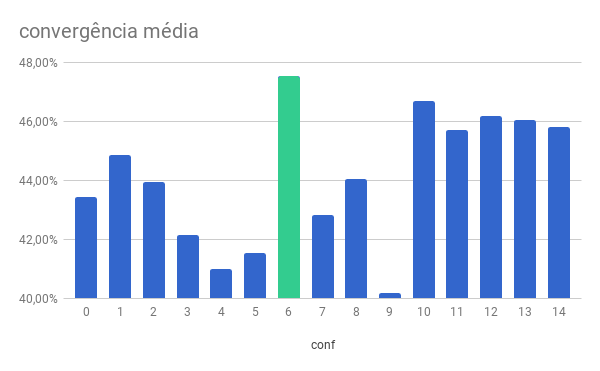
\includegraphics[width=0.40\textwidth]{conv1.png}} 
  \subcaptionbox*{}{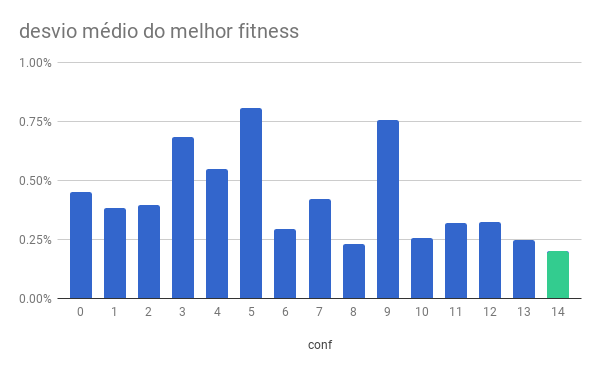
\includegraphics[width=0.40\textwidth]{best1.png}} \\
  \subcaptionbox*{}{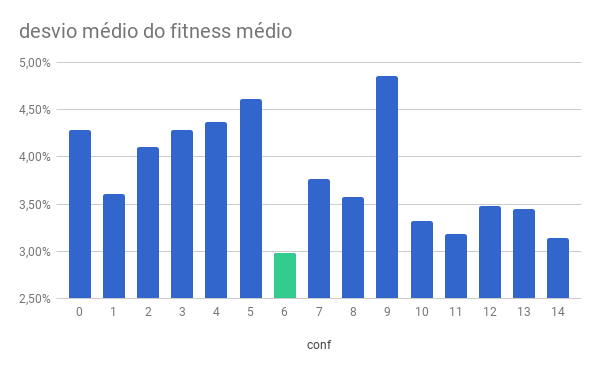
\includegraphics[width=0.40\textwidth]{mean1.png}} 
  \subcaptionbox*{}{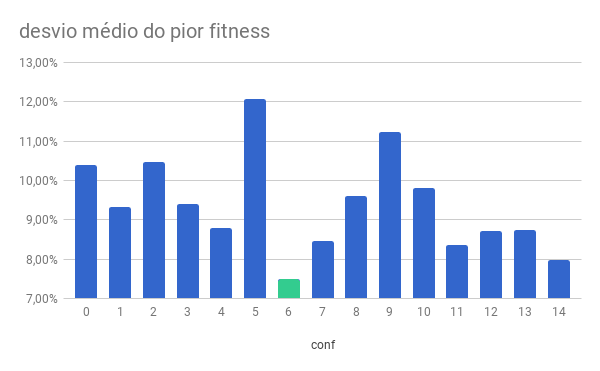
\includegraphics[width=0.40\textwidth]{worst1.png}} 
  \caption{Resultados agregados dos testes de configurações do AG para escalonamento de todos os grafos em 4 processadores. Os melhores resultados estão em destaque.}
  \label{fig:results1}
\end{figure*}

\begin{figure*}
  \centering
  \subcaptionbox*{}{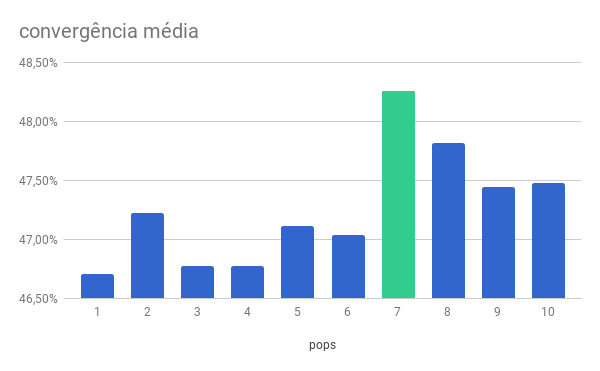
\includegraphics[width=0.40\textwidth]{conv2.png}} 
  \subcaptionbox*{}{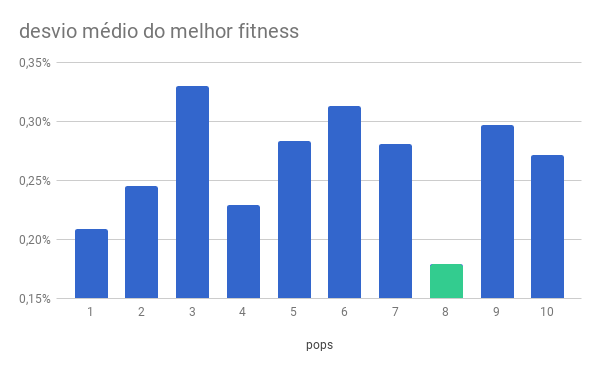
\includegraphics[width=0.40\textwidth]{best2.png}} \\
  \subcaptionbox*{}{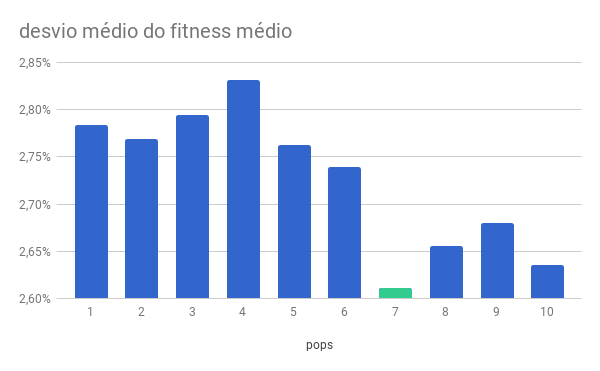
\includegraphics[width=0.40\textwidth]{mean2.png}} 
  \subcaptionbox*{}{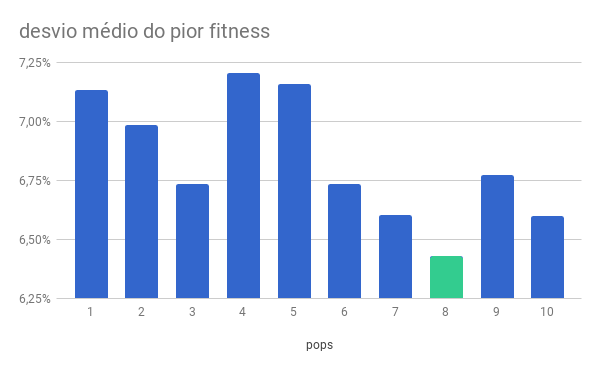
\includegraphics[width=0.40\textwidth]{worst2.png}} 
  \caption{Resultados agregados dos experimentos variando número de populações do AGMP para escalonamento de todos os grafos em 4 processadores. Os melhores resultados estão em destaque.}
  \label{fig:results2}
\end{figure*}


Em alguns dos experimentos, também nota-se que o AGMP encontrou soluções melhores do que as do AG com a configuração 6, como nos grafos fft39, fft95, laplace36 e random40, que são apresentados na Tabela \ref{tab:comp}. 
% \textbf{Entretanto, esses valores não superam os resultados considerados como ótimos (Tabela \ref{tab:opt}), obtidos por execuções do AG com parâmetros mais robustos.
% }

\begin{table}[h]
\centering
\caption{Melhor \textit{fitness} encontrado pelo AG e pelo AGMP com número de populações indicado, para 4 processadores.}
\label{tab:comp}
\begin{tabular}{|l|l|l|l|}
\hline
\textbf{grafo}     & \textbf{AG}   & \textbf{AGMP} & \textbf{populações} \\ \hline
fft39     & 840  & 820  & 8          \\ \hline
fft95     & 1620 & 1600 & 4          \\ \hline
laplace36 & 1300 & 1270 & 8          \\ \hline
random40  & 555  & 551  & 6          \\ \hline
\end{tabular}
\end{table}

% \begin{figure*}
%   \centering
%   \subcaptionbox*{}{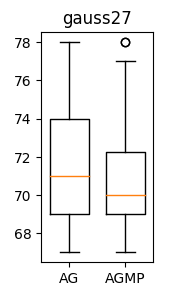
\includegraphics[width=0.24\textwidth]{boxplotgauss27}}
%   \subcaptionbox*{}{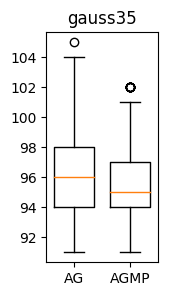
\includegraphics[width=0.24\textwidth]{boxplotgauss35}}
%   \subcaptionbox*{}{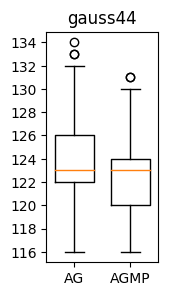
\includegraphics[width=0.24\textwidth]{boxplotgauss44}}
%   \subcaptionbox*{}{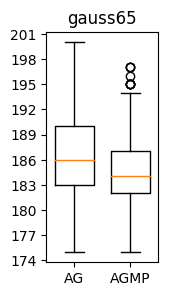
\includegraphics[width=0.24\textwidth]{boxplotgauss65}}
%   \\
%   \subcaptionbox*{}{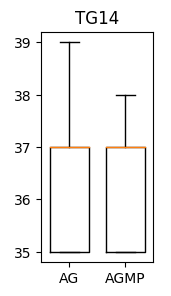
\includegraphics[width=0.24\textwidth]{boxplotTG14}}
%   \subcaptionbox*{}{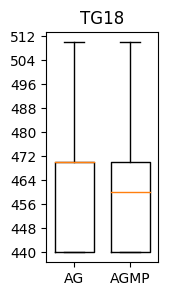
\includegraphics[width=0.24\textwidth]{boxplotTG18}}
%   \subcaptionbox*{}{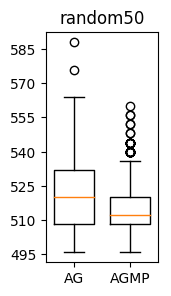
\includegraphics[width=0.24\textwidth]{boxplotrandom50}}
%   \subcaptionbox*{}{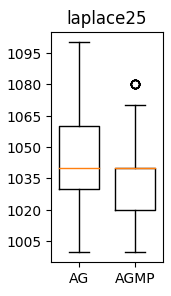
\includegraphics[width=0.24\textwidth]{boxplotlaplace25}}
%   \\
%   \subcaptionbox*{}{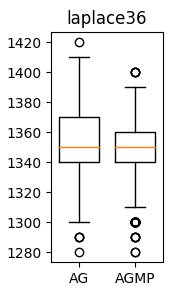
\includegraphics[width=0.24\textwidth]{boxplotlaplace36}}
%   \subcaptionbox*{}{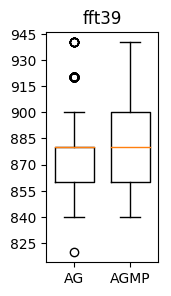
\includegraphics[width=0.24\textwidth]{boxplotfft39}}
%   \subcaptionbox*{}{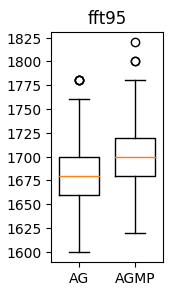
\includegraphics[width=0.24\textwidth]{boxplotfft95}}
%   \subcaptionbox*{}{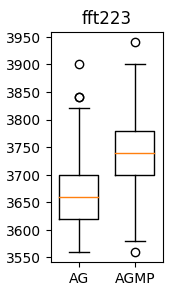
\includegraphics[width=0.24\textwidth]{boxplotfft223}}
%   \caption{ Boxplots dos valores de \textit{fitness} obtidos em $1000$ execuções do AG e do AGMP de 8 populações, considerando os grafos indicados e $4$ processadores. }
%   \label{fig:boxplots}
% \end{figure*}

% A Figura \ref{fig:boxplots} ilustra, através de boxplots, os resultados de $1000$ execuções do AG e do AGMP de 8 populações, omitindo os grafos em que não houve diferença entre o desempenho dos algoritmos. Nota-se que o AGMP foi mais consistente para a minimização do \textit{fitness} em oito dos doze grafos apresentados: TG14, TG18, random50, laplace25 e toda a família gauss. O AG serial obteve os melhores resultados para os grafos fft39, fft95 e fft223, embora o AGMP tenha sido capaz de encontrar escalonamentos com um \textit{makespan} melhor para o fft39 e o fft95 (Tabela \ref{tab:comp}).

A Tabela \ref{tab:hyp-test} mostra os resultados do teste de hipótese Wilcoxon Rank-Sum com significância de 95\%, que compara as medianas dos resultados obtidos pelo AGMP de 8 populações e pelo AG. Cada amostra é composta por $1000$ execuções. Foram considerados todos os grafos e, para avaliar se o desempenho relativo dos algoritmos se mantém para instâncias do problema com número diferente de processadores, foram consideradas as arquiteturas com $2$, $4$, $8$ e $16$ processadores, totalizando 104 cenários. Nota-se que o AGMP foi mais consistente para a minimização do \textit{fitness} em 44 cenários, se destacando para os grafos da família gauss, laplace16, laplace25, TG14, TG17 e TG18. O AG teve os melhores resultados em 19 cenários, com destaque para os grafos fft39, fft95, fft223 e random40. De modo geral, também pode-se observar que o desempenho relativo dos algoritmos se mantém para as instâncias do problema com número diferente de processadores.

Ao observar que o AGMP superou ou se equiparou ao AG em 85 dos 104 cenários, consideramos que os resultados suportam a hipótese de que o AGMP produz soluções melhores ou equivalentes às do AG no caso geral.

% Nota-se que o AGMP foi mais consistente para a minimização do \textit{fitness} em 11 dos 26 grafos: TG14, TG17, TG18, random50, laplace16, laplace25, laplace36 e toda a família gauss. O AG serial obteve os melhores resultados para os grafos TG12, random30, fft39, fft95 e fft223, embora o AGMP tenha sido capaz de encontrar escalonamentos com um \textit{makespan} melhor para o fft39 e o fft95 (Tabela \ref{tab:comp}).

% Para avaliar se o desempenho relativo dos algoritmos se mantém para instâncias do problema com número diferente de processadores, os experimentos foram executados considerando todos os grafos para arquiteturas com $2$, $4$, $8$ e $16$ processadores
% \begin{table}[]
% \label{tab:hyp-test}
% \caption{Resultados do teste de hipótese para as médias dos resultados do AGMP de 8 populações e do AG.}
% \begin{tabular}{|c|c|cc}
% \hline
% fft15                     & fft39                                  & \multicolumn{1}{c|}{fft95}                                  & \multicolumn{1}{c|}{fft223}                                 \\ \hline
% =                         & \cellcolor[HTML]{FE0000}\textgreater{} & \multicolumn{1}{c|}{\cellcolor[HTML]{FE0000}\textgreater{}} & \multicolumn{1}{c|}{\cellcolor[HTML]{FE0000}\textgreater{}} \\ \hline
% gauss27                   & gauss35                                & \multicolumn{1}{c|}{gauss44}                                & \multicolumn{1}{c|}{gauss65}                                \\ \hline
% \rowcolor[HTML]{34FF34} 
% \textless{}               & \textless{}                            & \multicolumn{1}{c|}{\cellcolor[HTML]{34FF34}\textless{}}    & \multicolumn{1}{c|}{\cellcolor[HTML]{34FF34}\textless{}}    \\ \hline
% laplace9                  & laplace16                              & \multicolumn{1}{c|}{laplace25}                              & \multicolumn{1}{c|}{laplace36}                              \\ \hline
% =                         & \cellcolor[HTML]{34FF34}\textless{}    & \multicolumn{1}{c|}{\cellcolor[HTML]{34FF34}\textless{}}    & \multicolumn{1}{c|}{\cellcolor[HTML]{34FF34}\textless{}}    \\ \hline
% TG4                       & TG9                                    & \multicolumn{1}{c|}{TG9b}                                   & \multicolumn{1}{c|}{TG10}                                   \\ \hline
% =                         & =                                      & \multicolumn{1}{c|}{=}                                      & \multicolumn{1}{c|}{=}                                      \\ \hline
% TG11                      & TG11b                                  & \multicolumn{1}{c|}{TG11c}                                  & \multicolumn{1}{c|}{TG12}                                   \\ \hline
% =                         & =                                      & \multicolumn{1}{c|}{=}                                      & \multicolumn{1}{c|}{\cellcolor[HTML]{FE0000}\textgreater{}} \\ \hline
% TG14                      & TG17                                   & \multicolumn{1}{c|}{TG18}                                   & \multicolumn{1}{c|}{random30}                               \\ \hline
% \rowcolor[HTML]{34FF34} 
% \textless{}               & \textless{}                            & \multicolumn{1}{c|}{\cellcolor[HTML]{34FF34}\textless{}}    & \multicolumn{1}{c|}{\cellcolor[HTML]{FE0000}\textgreater{}} \\ \hline
% random40                  & random50                               &                                                             &                                                             \\ \cline{1-2}
% \cellcolor[HTML]{FFFFFF}= & \cellcolor[HTML]{34FF34}\textless{}    & \cellcolor[HTML]{FFFFFF}                                    &                                                             \\ \cline{1-2}
% \end{tabular}
% \end{table}



\begin{table}[]
\centering
\caption{Testes de hipótese para as medianas dos resultados do AGMP de 8 populações e do AG. Os símbolos $<$, $=$ e $>$ indicam que a mediana do AGMP foi menor, igual ou maior que a do AG, respectivamente.}
\label{tab:hyp-test}
\begin{tabular}{c|c|c|c|c|}
\cline{2-5}
                                     & \multicolumn{4}{c|}{\textbf{processadores}}                                                                                                                       \\ \hline
\multicolumn{1}{|c|}{\textbf{grafo}} & \textbf{2}                             & \textbf{4}                             & \textbf{8}                             & \textbf{16}                            \\ \hline
\multicolumn{1}{|c|}{fft15}          & =                                      & =                                      & \cellcolor[HTML]{B7E1CD}\textless{}    & =                                      \\ \hline
\multicolumn{1}{|c|}{fft39}          & =                                      & \cellcolor[HTML]{F4C7C3}\textgreater{} & \cellcolor[HTML]{F4C7C3}\textgreater{} & \cellcolor[HTML]{F4C7C3}\textgreater{} \\ \hline
\multicolumn{1}{|c|}{fft95}          & \cellcolor[HTML]{B7E1CD}\textless{}    & \cellcolor[HTML]{F4C7C3}\textgreater{} & \cellcolor[HTML]{F4C7C3}\textgreater{} & \cellcolor[HTML]{F4C7C3}\textgreater{} \\ \hline
\multicolumn{1}{|c|}{fft223}         & =                                      & \cellcolor[HTML]{F4C7C3}\textgreater{} & \cellcolor[HTML]{F4C7C3}\textgreater{} & \cellcolor[HTML]{F4C7C3}\textgreater{} \\ \hline
\multicolumn{1}{|c|}{gauss27}        & \cellcolor[HTML]{B7E1CD}\textless{}    & \cellcolor[HTML]{B7E1CD}\textless{}    & \cellcolor[HTML]{B7E1CD}\textless{}    & \cellcolor[HTML]{B7E1CD}\textless{}    \\ \hline
\multicolumn{1}{|c|}{gauss35}        & \cellcolor[HTML]{B7E1CD}\textless{}    & \cellcolor[HTML]{B7E1CD}\textless{}    & \cellcolor[HTML]{B7E1CD}\textless{}    & \cellcolor[HTML]{B7E1CD}\textless{}    \\ \hline
\multicolumn{1}{|c|}{gauss44}        & \cellcolor[HTML]{B7E1CD}\textless{}    & \cellcolor[HTML]{B7E1CD}\textless{}    & \cellcolor[HTML]{B7E1CD}\textless{}    & \cellcolor[HTML]{B7E1CD}\textless{}    \\ \hline
\multicolumn{1}{|c|}{gauss65}        & \cellcolor[HTML]{B7E1CD}\textless{}    & \cellcolor[HTML]{B7E1CD}\textless{}    & \cellcolor[HTML]{B7E1CD}\textless{}    & \cellcolor[HTML]{B7E1CD}\textless{}    \\ \hline
\multicolumn{1}{|c|}{laplace9}       & =                                      & =                                      & =                                      & =                                      \\ \hline
\multicolumn{1}{|c|}{laplace16}      & =                                      & \cellcolor[HTML]{B7E1CD}\textless{}    & \cellcolor[HTML]{B7E1CD}\textless{}    & \cellcolor[HTML]{B7E1CD}\textless{}    \\ \hline
\multicolumn{1}{|c|}{laplace25}      & =                                      & \cellcolor[HTML]{B7E1CD}\textless{}    & \cellcolor[HTML]{B7E1CD}\textless{}    & \cellcolor[HTML]{B7E1CD}\textless{}    \\ \hline
\multicolumn{1}{|c|}{laplace36}      & \cellcolor[HTML]{F4C7C3}\textgreater{} & \cellcolor[HTML]{B7E1CD}\textless{}    & \cellcolor[HTML]{B7E1CD}\textless{}    & \cellcolor[HTML]{F4C7C3}\textgreater{} \\ \hline
\multicolumn{1}{|c|}{random30}       & \cellcolor[HTML]{F4C7C3}\textgreater{} & \cellcolor[HTML]{F4C7C3}\textgreater{} & \cellcolor[HTML]{B7E1CD}\textless{}    & =                                      \\ \hline
\multicolumn{1}{|c|}{random40}       & \cellcolor[HTML]{F4C7C3}\textgreater{} & =                                      & \cellcolor[HTML]{F4C7C3}\textgreater{} & \cellcolor[HTML]{F4C7C3}\textgreater{} \\ \hline
\multicolumn{1}{|c|}{random50}       & =                                      & \cellcolor[HTML]{B7E1CD}\textless{}    & \cellcolor[HTML]{B7E1CD}\textless{}    & =                                      \\ \hline
\multicolumn{1}{|c|}{TG4}            & =                                      & =                                      & =                                      & =                                      \\ \hline
\multicolumn{1}{|c|}{TG9}            & =                                      & =                                      & \cellcolor[HTML]{B7E1CD}\textless{}    & =                                      \\ \hline
\multicolumn{1}{|c|}{TG9b}           & =                                      & =                                      & =                                      & =                                      \\ \hline
\multicolumn{1}{|c|}{TG10}           & \cellcolor[HTML]{F4C7C3}\textgreater{} & =                                      & =                                      & \cellcolor[HTML]{F4C7C3}\textgreater{} \\ \hline
\multicolumn{1}{|c|}{TG11}           & =                                      & =                                      & =                                      & \cellcolor[HTML]{B7E1CD}\textless{}    \\ \hline
\multicolumn{1}{|c|}{TG11b}          & =                                      & =                                      & =                                      & =                                      \\ \hline
\multicolumn{1}{|c|}{TG11c}          & =                                      & =                                      & =                                      & =                                      \\ \hline
\multicolumn{1}{|c|}{TG12}           & =                                      & \cellcolor[HTML]{F4C7C3}\textgreater{} & \cellcolor[HTML]{B7E1CD}\textless{}    & \cellcolor[HTML]{B7E1CD}\textless{}    \\ \hline
\multicolumn{1}{|c|}{TG14}           & \cellcolor[HTML]{B7E1CD}\textless{}    & \cellcolor[HTML]{B7E1CD}\textless{}    & \cellcolor[HTML]{B7E1CD}\textless{}    & =                                      \\ \hline
\multicolumn{1}{|c|}{TG17}           & \cellcolor[HTML]{B7E1CD}\textless{}    & \cellcolor[HTML]{B7E1CD}\textless{}    & \cellcolor[HTML]{B7E1CD}\textless{}    & \cellcolor[HTML]{B7E1CD}\textless{}    \\ \hline
\multicolumn{1}{|c|}{TG18}           & \cellcolor[HTML]{B7E1CD}\textless{}    & \cellcolor[HTML]{B7E1CD}\textless{}    & \cellcolor[HTML]{B7E1CD}\textless{}    & \cellcolor[HTML]{B7E1CD}\textless{}    \\ \hline
\end{tabular}
\end{table}


%\begin{figure*}
 % \centering
  %\subcaptionbox*{}{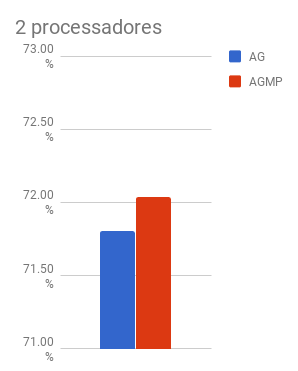
\includegraphics[width=0.24\textwidth]{2p}}
  %\subcaptionbox*{}{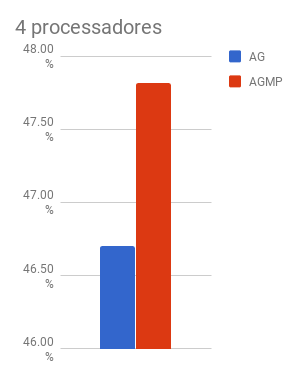
\includegraphics[width=0.24\textwidth]{4p}}
  %\subcaptionbox*{}{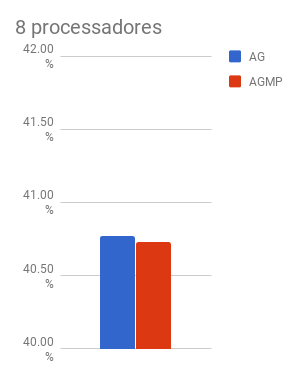
\includegraphics[width=0.24\textwidth]{8p}}
  %\subcaptionbox*{}{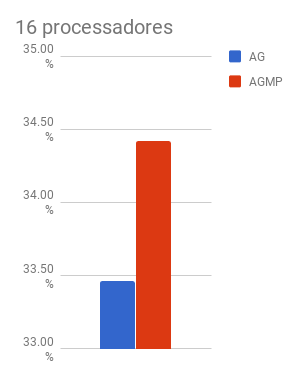
\includegraphics[width=0.24\textwidth]{16p}}
  %\caption{ Convergência média do AG e AGMP de 8 populações. }
%  \label{fig:convprocs}
%\end{figure*}

% \textbf{Para avaliar se o desempenho relativo dos algoritmos se mantém para instâncias do problema com número diferente de processadores, os experimentos foram executados considerando todos os grafos para arquiteturas com $2$, $4$, $8$ e $16$ processadores. A Figura \ref{fig:convprocs} mostra a convergência média do AG e do AGMP de 8 populações. Nota-se que a convergência média do AGMP iguala ou supera a do AG com exceção do caso de 8 processadores.}

\subsubsection{Tempo de execução}

Para avaliação de tempo de execução, foram usados os tempos gastos pelos experimentos da seção 5.4.1.  
%foram realizadas 100 execuções considerando o escalonamento de cada grafo em 4 processadores.
Os algoritmos evolutivos, implementados em linguagem C e otimizados pelo GCC, foram executados em um laptop com sistema operacional Ubuntu 16.04 e processador Intel Core i7-6500U, que possui $4$ núcleos e clock de 2,50GHz. Tal implementação proporcionou os tempos de execução médios dados na Tabela \ref{tab:time}, de acordo com o número de populações. Assim, foi calculado o \textit{Speedup} médio das configurações de AGMP, apresentado na Figura \ref{fig:speedup}, que mensura os desempenhos relativos ao tempo de execução do AG serial. O gráfico tem pico em $4$ populações e degrada em seguida, devido ao número de núcleos do processador utilizado, o que é previsto pela lei de Amdahl.

Considerando que o valor ideal de \textit{Speedup} é igual ao número de processos utilizado por um programa paralelo, nota-se que o \textit{overhead} relacionado ao procedimento de migração do AGMP teve impacto considerável sobre o seu tempo de execução. Por exemplo, o AGMP de $4$ populações obteve \textit{Speedup} de apenas $2,6$, sendo que, idealmente, seria $4$. Neste ponto, a configuração mais eficiente do AGMP foi a de $2$ populações, que obteve o maior \textit{Speedup} por número de processos.

Dado que o AGMP de 8 populações foi a configuração que obteve as soluções de melhor qualidade nos experimentos anteriores, nota-se que há um \textit{trade-off} entre qualidade das soluções e tempo de execução, uma vez que o \textit{Speedup} desta configuração foi inferior ao obtido pelas configurações supracitadas.

\begin{table}[h]
\centering
\caption{Tempo de execução médio dos experimentos, em milissegundos.}
\label{tab:time}
\begin{tabular}{|l|l|l|l|l|l|l|l|l|l|l|}
\hline
\textbf{populações} & 1     & 2     & 3     & 4     & 5     \\ \hline
\textbf{tempo (ms)} & 40,33 & 20,52 & 19,93 & 15,59 & 23,30 \\ \hline
\textbf{populações} & 6     & 7     & 8     & 9     & 10    \\ \hline
\textbf{tempo (ms)} & 21,93 & 23,67 & 23,00 & 22,89 & 23,26 \\ \hline
\end{tabular}
\end{table}

\begin{figure}[h]
\centering
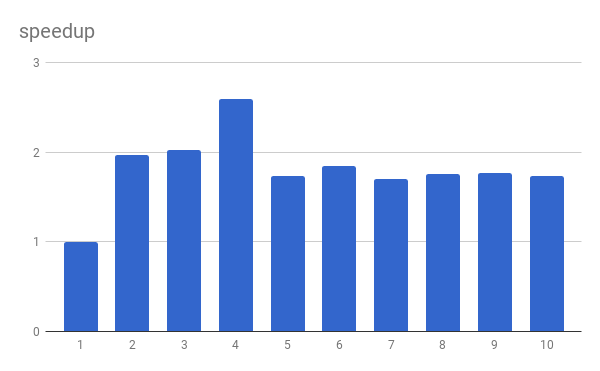
\includegraphics[width=0.5\textwidth]{speedup.png}
\caption{\textit{Speedup} por número de populações.}
\label{fig:speedup}
\end{figure}

É importante observar que os baixos tempos de execução apresentados na Tabela \ref{tab:time} não refletem o espaço de busca do problema. Na realidade, esses tempos são resultado da exploração de um número fixo de pontos de busca dado pelos parâmetros dos algoritmos evolutivos, como definido na seção \ref{sec:param}. Por exemplo, sendo $n$ o número de tarefas de um grafo, a cardinalidade do espaço de busca para o grafo laplace9 e 8 processadores é limitado entre \cite{Morady}: $P^n = 8^9 = 134.217.728$ e $n!P^n = 9! \cdot 8^9 = 48.704.929.136.640$, ou seja, este limite inferior é 2.571 vezes superior à quantidade de soluções avaliadas pelos algoritmos evolutivos neste trabalho. Para demonstrar experimentalmente a complexidade de se obter uma solução ótima para esta instância relativamente trivial, implementamos o algoritmo \textit{Branch and Bound}, que aplica uma árvore de busca e uma poda baseada no custo das tarefas restantes dividido pelo número de processadores. Ele foi implementado em linguagem Python, por proporcionar maior simplicidade de programação apesar de menor desempenho. Com este programa, após 76 minutos de execução e 414.473.362 avaliações de \textit{makespan}, foi obtido um \textit{makespan} de 520, o mesmo resultado obtido pelos algoritmos evolutivos com apenas 51.880 avaliações. Assim, verifica-se a capacidade destes de obter soluções ótimas mesmo com recursos consideravelmente reduzidos. Também pode-se verificar a relativa complexidade de se obter uma solução ótima mesmo para instâncias menores do problema e a necessidade do uso de métodos aproximados devido ao crescimento exponencial do espaço de busca.

% 414.473.362 avaliações


\section{Conclusões e Trabalhos Futuros}

% Neste estudo foi desenvolvido um AGMP para o problema de escalonamento de tarefas
Neste estudo, o desempenho do AGMP foi comparado com o do AG serial em relação ao problema de escalonamento de tarefas. Ambos foram desenvolvidos com a representação genética de dois vetores, que tem sido utilizada em trabalhos recentes. Foram implementados diversos métodos de \textit{crossover} adequados para cada vetor e, para a forma de sua aplicação, foram identificadas na literatura três abordagens diferentes, que foram implementadas e comparadas.

O desempenho do AGMP foi medido variando-se o número de populações e comparado com o desempenho do AG serial em termos de qualidade agregada das soluções e tempo de execução.

Foi composto um conjunto de grafos para \textit{benchmark} dos algoritmos, dividido entre grafos retirados da literatura e famílias de grafos baseadas em algoritmos reais. Para estas famílias, foram implementados scripts que geram grafos correspondentes à execução do algoritmo para diferentes tamanhos de entrada.

Os resultados suportam a hipótese de que AGMP é uma técnica que, dados parâmetros adequados, faz um melhor aproveitamento dos recursos computacionais disponíveis em comparação com o AG serial. Isto se dá de duas formas:

\begin{itemize}
\item Produção de soluções de mesma ou melhor qualidade para uma dada quantidade de avaliações de \textit{fitness}.
\item Redução do tempo de execução pelo uso de múltiplos núcleos dos processadores atuais.
\end{itemize}

Como trabalhos futuros, identificamos: realizar experimentos complementares com arquiteturas e grafos diferentes, e com variações do problema de escalonamento. Comparar o desempenho com outras abordagens de AG paralelo e outras meta-heurísticas, e.g. busca tabu \cite{Glover1999}, GRASP \cite{Feo1995} e VNS \cite{MLADENOVIC19971097}. Analisar a representatividade das formas de representação genética em relação às soluções alcançáveis no espaço de busca.

%Como trabalhos futuros, identificamos: realizar experimentos complementares, envolvendo escalonamento com alocação para arquiteturas com número de processadores diferente; comparar os resultados do AGMP com resultados da literatura; ampliar o repositório de \textit{benchmark} com base em algoritmos paralelos de relevância; avaliar um número maior de configurações para AG e AGMP, incluindo as combinações possíveis de métodos de \textit{crossover}, além de outros métodos para seleção e reinserção; avaliar \textit{Speedup} em máquinas com maior número de núcleos de processamento; analisar a convergência dos indivíduos ao longo das gerações; refinar o AGMP, investigando diferentes taxas de migração, frequências de migração, e topologias de comunicação; avaliar a dependência entre ajustes dessa parametrização e subconjuntos dos grafos do \textit{benchmark}, como famílias específicas ou grafos com número de vértices semelhante; investigar novas maneiras de implementação e modelos de paralelização de AG, como experimentos em cluster, AGs paralelos de fina granularidade baseados em vizinhança, e implementação para unidades de processamento gráfico (GPU); analisar a representatividade das formas de representação genética em relação às soluções alcançáveis no espaço de busca; implementar variações do escalonamento de tarefas, e.g. sistemas com processadores heterogêneos, com processadores em redes sem conexão total entre nós.



\section{Agradecimentos}

O presente trabalho foi realizado com apoio da Coordenação de Aperfeiçoamento de Pessoal de Nível Superior - Brasil (CAPES) - Código de Financiamento 001. Agradecemos a CAPES, CNPq e FAPEMIG pelo apoio financeiro que possibilitou esta pesquisa.

\section{Contribuição dos Autores}

\begin{itemize}
    \item Bruno W. Dantas Morais: desenvolvimento geral do trabalho.
    \item Gina M. Barbosa de Oliveira: orientação.
    \item Tiago Ismailer de Carvalho: co-orientação e estudo sobre as famílias de grafos.
\end{itemize} 

%----------------------------------------------------------------------------------------
%	REFERENCE LIST
%----------------------------------------------------------------------------------------

\phantomsection


\makeatletter
\renewcommand\@biblabel[1]{{\parbox{0.7cm}{[#1]}}}
\makeatother
% References
\renewcommand{\refname}{Referências}
\bibliography{refs}





\balance
\end{document}